% Paper 2A, version 19 (4 October 2026). Springer svjour3 class, prepared for
% the International Journal on Software Tools for Technology Transfer (STTT).
% Compile with pdflatex, bibtex, pdflatex, pdflatex. Requires svjour3.cls,
% svglov3.clo, spbasic.bst, and Paper_2A_Copied_Agreement_v19.bib in the same folder.
\RequirePackage{fix-cm}
\documentclass[smallextended,envcountsect,envcountsame,natbib]{svjour3}
\smartqed
\usepackage[utf8]{inputenc}
\usepackage[T1]{fontenc}
\usepackage{mathptmx}
\renewcommand{\ttdefault}{txtt}
\usepackage{amsmath,amssymb}
\usepackage{tikz,tikz-cd}
\usetikzlibrary{arrows.meta,positioning,shapes.geometric}
\usepackage{booktabs,array,tabularx,placeins,microtype}
\usepackage[hidelinks]{hyperref}
\usepackage{xurl}
\setlength{\emergencystretch}{3em}
\widowpenalty=10000
\clubpenalty=10000
\displaywidowpenalty=10000
\makeatletter
\setlength{\@fptop}{0pt}
\makeatother
\newcolumntype{L}{>{\raggedright\arraybackslash}X}
\newcommand{\code}[1]{\texttt{#1}}

\journalname{Int J Softw Tools Technol Transfer}

\begin{document}

\title{Copied Agreement: Lineage-Grounded Audits of\\ Claim Preservation in Data Migration}
\titlerunning{Copied Agreement}
\author{Duston Moore}
\authorrunning{D. Moore}
\institute{D. Moore \at
  Independent researcher, Edmonton, Alberta, Canada\\
  ORCID: 0009-0008-1103-9652
  % \\ \email{add contact address here}
}
\date{Received: date / Accepted: date}

\maketitle

\begin{abstract}
Equal outputs before and after a schema migration can reproduce a common error when the target is populated from an inadequate source. The audit given here separates three questions: whether the endpoints determine a claim, whether they agree on an exhibited carrier of migrated records, and whether they agree with a claim-relevant valuation whose production path is recorded. Four auditable conditions on a declared lineage graph expose production-path dependencies relevant to independent corroboration. Two are disclosure conditions: a shared dependency can be recorded while its defeater remains open. A countermodel shows a proposed ground satisfying the first three conditions while laundering shared coordinate ancestry. The fourth condition exposes that ancestry, and a fibre test decides whether the retained ground values factor through the retained ancestry values on the carrier. In a synthetic tax-jurisdiction migration with 1,728 seam records, endpoint comparison finds 48 disagreements, while comparison with delivery evidence finds 74 grounding witnesses. On 26 of these records both endpoints agree and both are wrong, found even though the old endpoint already fails to determine the claim. For a stably bound fixed ground, two lineage conditions compose across consecutive steps; the other two require stated ancestry conditions or a fresh outer audit. The fibre and seam lemmas are mechanised in Coq; the seam checks and the lineage and fibre decision cores are proved and extracted to OCaml behind tested wrappers. Positive assurance remains conditional on model relevance, carrier and lineage coverage, source fidelity, resolved defeaters, and custody.
\keywords{Data migration \and Data lineage \and Provenance \and Test oracles \and Assurance cases \and Coq}
\end{abstract}

\section{The claim made by a migration}\label{ex:sec:intro}
A schema migration often offers evidence of success in the form of equal outputs. The old and new implementations compute the same status on tested records, the dual write completes, and updating either side appears to commute with translation. The equality is real. Its relevance depends on the proposition the status is meant to establish and on the production of the two compared values. If the new field was populated from an inadequate old field, agreement can be a record of copying.

The audit developed here asks whether the inputs determine the promised claim, whether its old and new evaluations agree on the migrated records, and whether that agreement is supported by an independently produced ground. A positive answer to one question supplies no answer to the next.

\paragraph{Running example: a copied tax determination.} A synthetic retailer replaces a postal-zone field with a municipality field. Its old tax pipeline observes the zone, goods class, period, and charged rate. The new pipeline stores a municipality and applies a municipality-keyed table. Live rows are geocoded from the delivery address, but historical rows are backfilled by assigning the primary municipality of the old zone. Four zones also serve a secondary municipality. The concrete row
\[
(2,5,\mathit{general},\mathit{before},60)
\]
is the recurring counterexample. It records a delivery to municipality~5 in zone~2, but the backfill assigns zone~2's primary municipality. On this row the old flag and the copied new flag agree. A separately recorded delivery scan identifies municipality~5 and shows that their common result rests on the wrong jurisdiction. The paper reuses this row to separate four questions: whether the old observation can determine the jurisdictional claim, whether the old and new coordinates agree, whether a separately produced seam valuation agrees with them, and whether that valuation's production path is independent of both coordinates. Section~\ref{ex:sec:case} gives the complete executable case and its counts.

The distinction has a philosophical provenance, but none of the formal results depends on it.\footnote{A Whiteheadian motivation is that symbolic systems can remain internally orderly after their relation to the process has become defective, and that a settled record is not identical with the process from which it was produced \citep{whitehead1927symbolism,whitehead1929}. The engineering development replaces that motivation with tests stated in factorisation, provenance, lineage, coverage, and custody.}

\paragraph{Audience and practical rule.} The primary audience is data engineers, auditors, and formal-methods researchers who are responsible for claims, not merely records, that must survive a migration. The governing rule is that endpoint equality is not evidence that a claim survived a migration unless three conditions hold: the relevant observation surfaces determine the claim, the migration seam is exhibited with declared coverage, and the seam valuation has a production path that neither descends from either coordinate nor silently reuses their shared ancestry. Each obligation is developed separately, so that a failed claim has a location and a repair.

\paragraph{Contributions.} The paper makes four contributions. First, it decomposes claim preservation through migration into endpoint determination, seam coherence on an exhibited carrier, and grounded coherence against a lineage-qualified valuation, and it separates structural passing from certificate issuance (Sections~\ref{ex:sec:seams} and~\ref{ex:sec:evolution}). Second, it states lineage conditions (L1)--(L4) that make the production-path dependencies of a proposed ground auditable on a declared provenance graph. A countermodel shows that conditions on descent from the coordinates alone admit grounds that launder shared ancestry, and a fibre test detects extensional dependence on retained shared-ancestry values on a finite carrier (Section~\ref{ex:sec:laundering}). Third, it gives an exact composition analysis for a fixed ground: (L1) and (L4) compose across consecutive seams, while (L2) and (L3) carry over exactly under stated ancestry conditions, so a composite certificate needs either those conditions or a fresh outer audit (Section~\ref{ex:sec:lineage-composition}). Fourth, it supplies a Coq development of the exact core, extracted runtime checks, and a finite tax-jurisdiction audit in which the ground exposes 26 copied-agreement errors missed by endpoint comparison, with observational, stale-table, and backfill failures separated (Section~\ref{ex:sec:case}). The fibre criterion itself is a standard factorisation result; it serves as the observational baseline and is not claimed as a contribution.

\paragraph{Relation to the calculus companion.} \emph{Grounded Transport} develops a proof-relevant rewriting calculus for the same setting: witness identity and composition, algebraic laws, erasure, scopes, contexts, and evidence-bearing assessment \citep{moore2026transport}. This paper develops the migration diagnosis, the case study, and the lineage conditions and their composition. The accompanying metric supplement keeps the bounded-error extensions separate from the exact audit. Composing already certified calculus witnesses does not establish that an unexamined outer coordinate pair satisfies the migration lineage conditions: the calculus carries supplied evidence, whereas this paper asks which evidence the migration must supply. The companion's pinned implementation checks (L1)--(L3), not (L4), and mechanises analogous fixed-ground composition results with different countermodels (Section~\ref{ex:sec:lineage-composition}). Each paper states the shared definitions it needs; their contributions and verification evidence are separate.

\paragraph{Scope.} The paper does not propose a general semantics for relational databases, a complete SQL-equivalence procedure, a probabilistic calibration theorem, or a proof that a concrete process has been exhaustively captured. Its mechanisation has three layers. The pinned baseline covers constructive exact factorisation, the seam grounding equations and their witness refutations, and certified evolution; exhibition and lineage enter its transport definition as abstract premises, and its finite factor-table checker and tax lineage audit are handwritten OCaml. The companion's separately pinned implementation mechanises the single-seam conditions (L1)--(L3), including the strengthened identity and directly raw ground cases \citep{moore2026transport}. The extension mechanises (L4) disclosure and its composition, the exact (L2) coverage and (L3) source-survival conditions, the paper's two finite countermodels, and a finite fibre checker with proved witness soundness, factor soundness, and non-certification on incomplete carriers. Its lineage and retained-value decision cores are extracted to OCaml; string encoding, retention validation, and output formatting remain handwritten and tested. The metric supplement and the assurance predicates lie outside the mechanisation.

\paragraph{Organisation.} Section~\ref{ex:sec:related} relates the audit to migration testing, differential testing, truth discovery, and provenance. Section~\ref{ex:sec:static} states the static baseline and the vocabulary of application warrant. Section~\ref{ex:sec:seams} introduces the migration seam, grounding, and the lineage conditions, and Section~\ref{ex:sec:evolution} treats evolution and composition. Section~\ref{ex:sec:observational} describes how endpoint evidence enters the audit and gives the finite reference procedure. Section~\ref{ex:sec:case} works the tax case, Section~\ref{ex:sec:practice} gives the practical procedure, and Sections~\ref{ex:sec:limitations} and~\ref{ex:sec:conclusion} state limitations and conclude.

\begin{table}[htbp]
\centering
\small
\caption{Core notation.}
\label{ex:tab:notation}
\begin{tabularx}{\textwidth}{@{}p{2.8cm}L@{}}
\toprule
Symbol & Meaning \\
\midrule
$S$, $S_t$ & Declared state model, or the state model at stage $t$ \\
$M:S\to O$ & Observation map from states to the declared observation surface \\
$\Phi:S\to 2$ & Exact predicate whose determination is claimed \\
$\chi$; $\chi_t$ & Declared claim, and its evaluation on the stage-$t$ state model \\
$A_t,B_t$ & Concurrent old and new coordinate models at window stage $t$ \\
$R_t$ & Migration seam carrier accountable under both coordinate descriptions \\
$p_t,q_t$ & Projections from the seam carrier to old and new coordinate state models \\
$\Phi_{R,t}$ & Claim-relevant valuation evaluated on the seam from process evidence \\
$L$ & Declared finite lineage graph for the coordinate and seam valuations \\
$\operatorname{Raw}(L)$, $\operatorname{Rel}(L)$ & Declared raw lineage nodes, and the subset marked claim-relevant \\
$\operatorname{anc}(x)$ & Strict ancestors of node $x$ in the lineage graph \\
$D$ & Shared non-raw ancestry of the two coordinate determinations \\
$E_g$ & Non-raw ancestry shared by the ground and either coordinate \\
\bottomrule
\end{tabularx}
\end{table}

\section{Background and related work}\label{ex:sec:related}\label{ex:sec:formal-neighbours}

\paragraph{Migration testing and data validation.} Standard migration methodology defines correctness relative to the source. Data validation compares source and target databases, and reconciliation maps source identifiers to target identifiers to establish completeness \citep{matthesschulzhaller2011}. The same literature requires reconciliation code to be written afresh rather than copied from the transformation programs it tests, so that their errors are not repeated. Declarative data-quality checking extends such tests to production pipelines: Deequ, for example, lets engineers state constraints and metrics over large datasets and verifies them incrementally \citep{schelter2018}. These methods test fidelity to a source or to declared constraints. They do not ask whether a value faithfully copied from the source was ever correct for the claim it supports. The lineage conditions of Section~\ref{ex:sec:grounding-seam} extend the independence requirement from the checking code to the evidence against which the migrated claim is checked.

\paragraph{Differential testing and the oracle problem.} Comparing old and new evaluations is a form of differential, or back-to-back, testing: comparable systems are run on the same inputs and their disagreements are investigated \citep{mckeeman1998}. Its known limitation is that two systems sharing a fault agree on it. Deciding whether an agreed output is correct is the test-oracle problem \citep{barr2015}. In these terms, seam coherence (Definition~\ref{ex:def:seamcoherence}) is differential testing on the migrated records, and grounded coherence (Definition~\ref{ex:def:grounded-seam}) is oracle-based testing in which the oracle's independence from the systems under test is itself audited over a provenance graph.

\paragraph{Independence of versions and sources.} Knight and Leveson showed experimentally that independently developed versions of one specification do not fail independently \citep{knightleveson1986}. The same point applies to evidence: two separately maintained instruments can share a blind spot. The conditions here concern production-path independence for corroboration; they do not establish independence of failure. In data integration, truth-discovery methods recognise that copying among sources inflates apparent agreement. Dong, Berti-\'Equille, and Srivastava model copying between sources and infer it from shared values, particularly shared false values, so that copied agreement is discounted when deciding which value is true \citep{dong2009}. That work detects dependence statistically across many sources. The present audit instead requires the dependence structure of one seam valuation to be declared and checks it. The two are complementary: statistical copy detection can challenge a declared graph that claims independence, and a declared graph can explain why agreement observed on a carrier should not be counted as corroboration.

\paragraph{Belief merging and repeated sources.}
In the framework of Konieczny and Pino P\'erez, the source profile
is a multiset, allowing repeated beliefs from distinct sources to
affect merging \citep{konieczny2002merging}. Where reports repeat
a common upstream claim, source multiplicity alone does not establish
independent corroboration. The present audit addresses the declared
production paths relevant to that evidential distinction; it does
not define a new belief-merging operator.

\paragraph{Provenance.} Database provenance distinguishes why an output appears from where its values were copied \citep{buneman2001}, and provenance semirings preserve alternative and joint derivations through relational queries \citep{greenkarvounarakistannen2007}. The W3C PROV data model supplies a standard vocabulary for entities, activities, agents, generation, use, and derivation \citep{w3cprovdm2013}. These supply the graph. Conditions (L1)--(L4) are additional, claim-specific constraints over it (Section~\ref{ex:sec:grounding-seam}).

\paragraph{Online schema change.} Production systems change schemas while serving traffic by passing through intermediate schema states that keep concurrently running servers consistent \citep{rae2013}. Such protocols govern when old and new representations may coexist and how data is backfilled. They make the seam carrier of Section~\ref{ex:sec:migration-seam} concrete, but they do not address whether a backfilled value is true of the occurrence it describes.

\paragraph{Categorical data migration.} Functorial data migration models a schema as a small category, an instance as a set-valued functor, and a schema functor as inducing canonical data-migration functors \citep{spivak2012,spivakwisnesky2012}. The seam used here is a different object. $R_t$ is a carrier of process or record instances accountable under both descriptions, and its projections relate those instances to the two coordinate state models. A categorical migration may implement or justify parts of the projections or an observational translation, but categorical preservation alone does not answer whether the carried value has a claim-relevant ground independent of the source coordinate.

\paragraph{Query and application equivalence.} Database verification supplies stronger proof techniques when the relevant semantics can be expressed symbolically. Cosette combines constraint-based counterexample search with proof-assistant reasoning for SQL query equivalence \citep{chucosette2017}; Q*cert mechanises semantics and correctness properties for query-compilation pipelines in Coq \citep{auerbach2017}; and Mediator uses bisimulation invariants to verify equivalence of database-driven applications across schema changes \citep{wang2018}. These methods can discharge obligations that a finite enumeration cannot. They do not, by themselves, establish the completeness of a seam carrier, the independence of a claimed ground, or the accuracy of the raw process evidence. Conversely, the fibre and grounding criteria do not replace query or program equivalence when those are the claims at issue.

\paragraph{Assurance arguments.} Assurance~2.0 treats assurance as an eliminative argument in which identified defeaters must be answered or left explicitly open \citep{bloomfieldrushby2021,bloomfieldnetkachovarushby2024}. The witnesses defined below fit that structure, and the disclosure conditions (L2) and (L4) record defeaters rather than resolve them.

\paragraph{Formal neighbours of the fibre criterion.} The factorisation test of Section~\ref{ex:sec:test} has established relatives: measurable factorisation in the Doob--Dynkin lemma \citep[Lemma~1.13]{kallenberg2002}, Blackwell's comparison of experiments \citep{blackwell1953}, the data-processing inequality \citep{coverthomas2006}, exactness of the Galois abstraction induced by an observation map \citep{cousot1977}, and noninterference when the state space is a product and the observer sees one component \citep{goguenmeseguer1982}. A companion manuscript develops these relations \citep{moore2026exactness}; none is claimed as a contribution here.

\paragraph{Position.} The requirement that a check be independent of what it checks is old. The contribution here is to state that requirement for the evidence used to corroborate a migrated claim, as conditions on a declared lineage graph that can be checked, composed, and reported with their residual assumptions, and to show on a worked case what they detect that endpoint comparison does not.

\section{Claims, observation surfaces, and application warrant}\label{ex:sec:static}

\subsection{Application warrant and continuing reliance}\label{ex:sec:warrant}

\begin{definition}[Application warrant]\label{ex:def:warrant}
Application warrant is the evidential entitlement to assert a specified claim about a concrete case for a stated use and time, conditional on the adequacy of the artefact's construction and on the continuing operation of practices that preserve its claim-relevant distinctions.
\end{definition}

A passing internal check supplies only part of that entitlement. The state model, observation map, and predicate must fit the claim; the observation must determine it; and the instruments, transformations, and evidence must remain adequate after change. Factorisation establishes the determination condition within the declared model. It does not establish the relevance of that model or the fidelity of the instruments that realise it. The justification for those initial choices is \emph{construction warrant}.

\emph{Warrant Debt} is continued institutional reliance on a claim while a necessary condition of its application warrant remains unmet. A defect found and repaired before reliance is not debt. The tax case locates unmet conditions in construction, observation, maintenance, and institutional custody so that each repair has an evidential basis and an owner. The wider account is developed separately \citep{moore2026exactness}; the present audit identifies failures and does not infer continued reliance from a witness alone.

A claim is \emph{affirmed} for a declared scope when its warrant conditions are established, \emph{denied} when evidence refutes it, and \emph{underdetermined} otherwise. A clean search supports affirmation only when it is complete for the asserted scope.

\subsection{Static baseline: observation-relative admissibility}\label{ex:sec:test}

The surface $M$ identifies states with the same observed value. Exact determination of $\Phi$ requires $\Phi$ to respect that identification. The test compares the declared map and predicate; it does not establish that either fits the concrete process $\mathcal{C}$.

\subsubsection{The domain}

The model $S$ already embodies choices about occurrences and relevant differences. Let $\mathcal{C}$ be the concrete process, $\iota$ its modelling as $S$, and $M:S\to O$ the declared observation map:
\[
\mathcal{C} \overset{\iota}{\longrightarrow} S \overset{M}{\longrightarrow} O.
\]
The test below concerns whether the predicate $\Phi:S\to 2$ survives $M$. It does not test the placement of $\iota$ or the accuracy of an implemented observation. Examples of $\Phi$ include tenant isolation and the absence of a forbidden transition.

\paragraph{The concrete process is not an oracle.} The notation $\mathcal{C}$ names the process about which the regime makes its claim; it does not assume unmediated access to ``ground truth''. Every operational check reaches the process through instruments, traces, scans, source records, or other evidence. Those records can themselves be wrong or incomplete. The formal results are therefore conditional in two ways. Factorisation asks whether a declared representation preserves the distinctions required by a declared predicate. Grounded migration asks whether the seam valuation has a claim-relevant production path independent of the two coordinates. Neither establishes the accuracy or completeness of the evidence at the start of that path. Those are construction and institutional obligations, and a positive formal result must retain them as stated assumptions.

\begin{definition}[Observation-relative admissibility]\label{ex:def:admissible}
$\Phi$ is $M$-admissible, written $\operatorname{Admissible}_M(\Phi)$, when $\Phi=\widehat\Phi \circ M$ for some map $\widehat\Phi:O\to 2$.
\end{definition}

\paragraph{Engineering reading.} If two concrete cases look identical on the complete input surface $M$, they must require the same answer to the exact claim $\Phi$. In the running example, the old zone-based surface cannot distinguish an order delivered to zone~2's primary municipality from an otherwise identical order delivered to municipality~5. Since the correct jurisdictional answer differs, the old surface cannot determine that claim exactly.

\paragraph{Why this formalism?} The promised relation is exact recovery of $\Phi$ from the complete declared input $M(s)$. States identified by $M$ must then have the same $\Phi$ value. Factorisation tests that requirement. Predictive accuracy is a different property: a predictor may perform well even though one observation fibre contains states with different target values.

Over arbitrary $S$ and $O$, admissibility asserts existence rather than computability. The finite procedure of Section~\ref{ex:sec:finite-procedure} constructs a factor only with a certified complete enumeration of $S$ and decidable equality on $O$. Exact determination from $M$ entails admissibility; admissibility alone does not warrant application:
\[
\text{warrant for exact $M$-based determination of $\Phi$} \;\Longrightarrow\; \operatorname{Admissible}_M(\Phi).
\]
A calibrated estimate does not promise to determine each individual's $\Phi$ and need not satisfy this condition. A computed score $f(M(s))$ trivially factors through $M$ as a score; that does not establish calibration to an outcome or justify an adverse decision. Those claims require an identified outcome and use, sampling and error evidence, and review after changes in population or features. If a score is used as an exact individual determination, that stronger claim must satisfy the fibre test.

The following lemma is standard; it is the universal property of the quotient of $S$ by the kernel of $M$, and everything later depends on it.

\begin{lemma}[Fibre criterion]\label{ex:prop:fibre}
$\Phi$ is $M$-admissible if and only if, for all $s_1,s_2 \in S$, $M(s_1)=M(s_2)$ implies $\Phi(s_1)=\Phi(s_2)$.
\end{lemma}

\begin{proof}
If $\Phi=\widehat\Phi \circ M$ and $M(s_1)=M(s_2)$, then $\Phi(s_1)=\widehat\Phi(M(s_1))=\widehat\Phi(M(s_2))=\Phi(s_2)$. Conversely, suppose $\Phi$ is constant on every fibre of $M$. Define $\widehat\Phi(o)=1$ when some $s \in S$ satisfies $M(s)=o$ and $\Phi(s)=1$, and $\widehat\Phi(o)=0$ otherwise. If $\Phi(s)=1$, the defining condition holds at $M(s)$. If $\Phi(s)=0$, fibre constancy excludes any $s'$ with $M(s')=M(s)$ and $\Phi(s')=1$. Hence $\widehat\Phi(M(s))=\Phi(s)$ for every $s$.\qed
\end{proof}

\begin{remark}[Constructive qualification]
The converse is classical: the definition of $\widehat\Phi$ decides an existential. In constructive type theory, fibre constancy does not supply that decision; a complete enumeration, decidable equality, an explicit section, or a classical axiom must be added. The accompanying repository contains the checked constructive version, and Appendix~\ref{ex:app:verification} reports its assumptions. In classical set theory the criterion holds for any nonempty codomain in place of $2$: choose a representative on each nonempty fibre and a default value off the image. Sections~\ref{ex:sec:laundering} and~\ref{ex:sec:debt-extensions} use this generalisation.
\end{remark}

A witness refutes admissibility. A factorisation proof or complete finite check establishes it within the declared model. An incomplete clean search returns \code{NoWitnessFound}: an unresolved assessment, not a positive certificate, in keeping with Dijkstra's observation about testing \citep{dijkstra1970}.

\begin{definition}[Observational witness]\label{ex:def:witness}
An observational witness for $(M,\Phi)$ is a pair $s_1,s_2 \in S$ with $M(s_1)=M(s_2)$ and $\Phi(s_1) \neq \Phi(s_2)$.
\end{definition}

\paragraph{Engineering reading.} A witness is a two-row counterexample: the system sees the same declared inputs but the promised exact answer differs. The running case supplies the pair $(2,2,\mathit{general},\mathit{before},60)$ and $(2,5,\mathit{general},\mathit{before},60)$. No downstream function of the old surface alone can recover which municipality received the order.

\begin{proposition}[No recovery by post-processing]\label{ex:prop:norecovery}
Let $f:O\to Y$ be any map. If $M(s_1)=M(s_2)$, then $(f \circ M)(s_1)=(f \circ M)(s_2)$. Hence no procedure whose input is only $M(s)$ recovers a distinction that $M$ identifies.
\end{proposition}

\begin{proof}
Apply $f$ to both sides of $M(s_1)=M(s_2)$.\qed
\end{proof}

\begin{remark}[Randomised post-processing]\label{ex:cor:no-stochastic-recovery}
The same holds for a randomised procedure. If $K:O\to\mathcal{P}(Y)$ assigns to each observation the output distribution of a possibly randomised post-processor, where $\mathcal{P}(Y)$ is the set of probability distributions on $Y$, then $K(M(s_1))=K(M(s_2))$ at any observational witness, so no such procedure distinguishes the two witness states by their output laws.
\end{remark}

Write $\ker M$ for the equivalence relation $\{(s_1,s_2)\in S\times S\mid M(s_1)=M(s_2)\}$. Lemma~\ref{ex:prop:fibre} says that $\Phi$ is $M$-admissible if and only if $\ker M \subseteq \ker \Phi$, which locates the minimal formal repair.

\begin{proposition}[Coarsest admissible refinement]\label{ex:prop:shell}
For any map $M':S\to O'$, $\Phi$ is $M'$-admissible if and only if $\ker M' \subseteq \ker \Phi$. In particular, among maps whose kernels refine $\ker M$, the coarsest kernel on which $\Phi$ is admissible is $\ker \langle M,\Phi \rangle=\ker M \cap \ker \Phi$.
\end{proposition}

\begin{proof}
The first claim is Lemma~\ref{ex:prop:fibre}. If $\ker M' \subseteq \ker M$, then $\ker M' \subseteq \ker \Phi$ holds if and only if $\ker M' \subseteq \ker M \cap \ker \Phi$, and $\ker M \cap \ker \Phi=\ker \langle M,\Phi \rangle$ is itself admissible.\qed
\end{proof}

For abstraction domains induced by partitions, Proposition~\ref{ex:prop:shell} is a one-predicate case of complete-shell refinement \citep{giacobazziranzatoscozzari2000,ranzatotapparo2004}: adding the truth set of $\Phi$ splits exactly the mixed blocks of $M$. The proposition identifies the minimal formal refinement, not an observation that can be built. The surface $\langle M,\Phi \rangle$ presupposes an instrument that observes $\Phi$. A regime can refine only by maps it can realise, so the minimal realisable refinement may be strictly finer than $\ker M\cap\ker\Phi$; which refinement it can instrument is a question of construction warrant.


\section{Seams and grounded coherence}\label{ex:sec:seams}\label{ch:change}

The dynamic analysis has four steps. First, it asks whether an earlier certificate remains applicable after change. Second, it exhibits the migration seam and tests extensional seam coherence. Third, it strengthens that test with coherence against a lineage-qualified valuation. Fourth, Section~\ref{ex:sec:evolution} checks whether the seam and its coordinate descriptions evolve functorially across the declared interval, and how seams compose. These obligations are cumulative: success at a later step does not repair failure at an earlier one. Throughout, continuity means preserving the distinctions on which a claim depends, not merely retaining a value or copying a record.

\subsection{Dynamic admissibility}\label{ex:sec:dynamic}

\begin{definition}[Dynamic observation regime]
A dynamic observation regime is a family $\{M_t:S_t\to O_t\}_{t \in T}$, indexed by a linearly ordered set of stages $T$ in which each non-final stage $t$ has an immediate successor $t+1$, together with transition data $\Gamma_t$ for each consecutive pair. The data $\Gamma_t$ relate $(S_t,M_t,\Phi_t)$ to $(S_{t+1},M_{t+1},\Phi_{t+1})$: they comprise a span relating the two state models (defined below), the change of observation surface, and the change, if any, of the predicate.
\end{definition}

\paragraph{Engineering reading.} Treat each deployment stage as a versioned observation contract. The transition record must say what changed in the state model, which fields or instruments changed, and whether the claim itself changed. A schema version number alone is not enough.

The transition data are a record, not a morphism in a category of regimes; no such category is needed. The only mathematical structure imposed on them is the span of Section~\ref{ex:sec:migration-seam} and the evolution maps of Section~\ref{ex:sec:functorial-transport}. The stages need not describe a single monolithic cut-over. Rolling deployments, dual-write periods, and distributed services can be represented by successive stages and overlapping seam carriers, provided the claim-bearing records, their coverage, and their responsible custodians are declared. The framework does not require synchronous consistency or one central database; it requires an auditable relation for the claim being transported.

\begin{definition}[Warrant Debt after a transition]\label{ex:def:dynamic-debt}
An institution incurs Warrant Debt when it continues to rely on the assertion of $\Phi_{t+1}$ for a specified use while an unmet condition of application warrant persists, for example when it carries an earlier certificate across a change that removed a distinction required by $\Phi_{t+1}$.
\end{definition}

\paragraph{Engineering reading.} A detected migration defect is a repair item. It becomes Warrant Debt when the organisation keeps using the affected determination while the required evidence or repair remains open.

\begin{corollary}[Dynamic fibre criterion, fixed state model]\label{ex:cor:dynfibre}
Let $S$ be common to stages $t$ and $t+1$, with maps $M_t:S\to O_t$ and $M_{t+1}:S\to O_{t+1}$, and let $\Phi_{t+1}:S\to 2$. A certificate for $\Phi_{t+1}$ that uses only $M_t$ is admissible if and only if $\Phi_{t+1}$ is constant on every fibre of $M_t$.
\end{corollary}

\begin{proof}
Lemma~\ref{ex:prop:fibre} with $\Phi_{t+1}$ for $\Phi$ and $M_t$ for $M$.\qed
\end{proof}

\begin{proposition}[Certificate expiry]\label{ex:prop:certificate-expiry}
An admissibility certificate is regime-indexed: in general,
\[
\operatorname{Admissible}_{M_t}(\Phi_t)
\not\Longrightarrow
\operatorname{Admissible}_{M_{t+1}}(\Phi_{t+1}).
\]
The non-implication already occurs (a) when the later surface is an information-losing coarsening and the predicate is unchanged, and (b) when the surface is unchanged and the predicate is redefined.
\end{proposition}

\begin{proof}
For (a), let $S=2$, $M_t=\operatorname{id}_2$, $M_{t+1}$ be constant, and $\Phi_t=\Phi_{t+1}=\operatorname{id}_2$. The stage-$t$ predicate is admissible, while $0$ and $1$ form an observational witness at $t+1$. For (b), let $S=2$ again, let both surfaces be the constant map $S\to\{*\}$, let $\Phi_t$ be constant, and let $\Phi_{t+1}=\operatorname{id}_2$. Again the earlier predicate is admissible and the later one is not.\qed
\end{proof}

Not every change destroys admissibility: an unchanged $\Phi$ remains admissible if $M_{t+1}$ distinguishes at least what $M_t$ did. The actual transition, however, must be checked before the earlier certificate is used. Continued reliance without that review may incur maintenance Warrant Debt (Section~\ref{ex:sec:warrant}).

\subsection{The migration seam}\label{ex:sec:migration-seam}

In the running tax example, a seam element is one order represented under both schemas during the migration window. Live dual-writes and historical backfill rows are different seam origins because they have different production paths. The seam therefore records not only which old and new rows correspond, but how the corresponding pair entered the migration.

When a system is re-architected, old and new states are not the same objects, and relating $S_t$ to $S_{t+1}$ requires a span
\[
S_t \xleftarrow{\;p_t\;} R_t \xrightarrow{\;q_t\;} S_{t+1}.
\]
Here $R_t$ records the pieces of process accountable to both an old state and a new one, such as a request in flight during a deployment or a record migrated and not yet re-indexed. In an online schema migration from a free-text address field to a structured one, a request that dual-writes during the migration window is an element of $R_t$, read under the old shape by $p_t$ and committed under the new shape by $q_t$. A runbook that logs its dual-written requests exhibits $R_t$; one that does not leaves the claim that certificates survived the migration without an object on which to check it.

This set-level span is the audit object; Section~\ref{ex:sec:related} contrasts it with categorical data migration.

\begin{definition}[Exhibited seam]\label{ex:def:exhibited-seam}
A migration seam for a claim consists of (a) a mathematical span
\[
S_t\xleftarrow{p_t}R_t\xrightarrow{q_t}S_{t+1},
\]
and (b) an assurance record $\rho_t$. It is \emph{exhibited} when the record supplies (i) stable identifiers for the relevant carrier elements; (ii) provenance linking each element through $p_t$ and $q_t$ to one declared process; (iii) evidence sufficient to evaluate the claim-relevant seam valuation; (iv) a coverage declaration for the transition interval, including relevant occurrences not represented in $R_t$; and (v) an authorised custodian responsible for retention and review. The span alone establishes none of these record conditions.
\end{definition}

\begin{definition}[Declared coverage]\label{ex:def:coverage}
For a claim $\chi$ and transition interval $I$, let $\Omega$ be the declared occurrence model and let $C\subseteq\Omega\times I$ be the scope on which the claim is asserted. A coverage declaration identifies $(\chi,I,C)$, the rule assigning carrier records to occurrences in $C$, exclusions, and known or unresolved gaps. A result is reported as a result on $C$ relative to that declaration. It is not extended to a larger population or interval without new evidence.
\end{definition}

The declaration must distinguish exclusions outside the asserted scope from missing cases inside it. Narrowing the claim to a supported subset changes $C$; it does not prove the excluded claim. Completeness of the declared occurrence model, coverage of the carrier, and coverage of the production graph remain different obligations.

\paragraph{Engineering reading.} The auditor needs an inspectable migration population, not merely two endpoint tables. For the tax case this means stable order identifiers, the old and new records for each covered order, enough delivery evidence to evaluate the jurisdictional check, explicit inclusion and exclusion rules for the cut-over window, and a named owner of the record.

Exhibition requires a record, not proof that $R_t$ exhausts the process. Condition (iii) says only that the seam valuation can be evaluated from the record; lineage independence is separate (Definition~\ref{ex:def:lineage-qualified-three}). A broken identity link, unevaluable valuation, uncovered class, or missing custodian defeats exhibition. The record's capacity to support its valuation is itself a factorisation obligation; a missing coverage record leaves that obligation unmet.

The custodian is an institutional role, not a mathematical witness. For the assurance record to be reviewable, it should name the custodian's scope of authority, access to the relevant evidence, responsibility for retention and revalidation, and the route by which unresolved coverage or lineage defects are escalated. Separation from the migration implementation helps to avoid a shared failure mode, but independence must be evidenced, not inferred from a job title. The checker can inspect whether these declarations exist and whether an assigned role has the stated authority; it cannot prove competence, adequate resources, good faith, or future performance.

\begin{figure}[htbp]
\centering
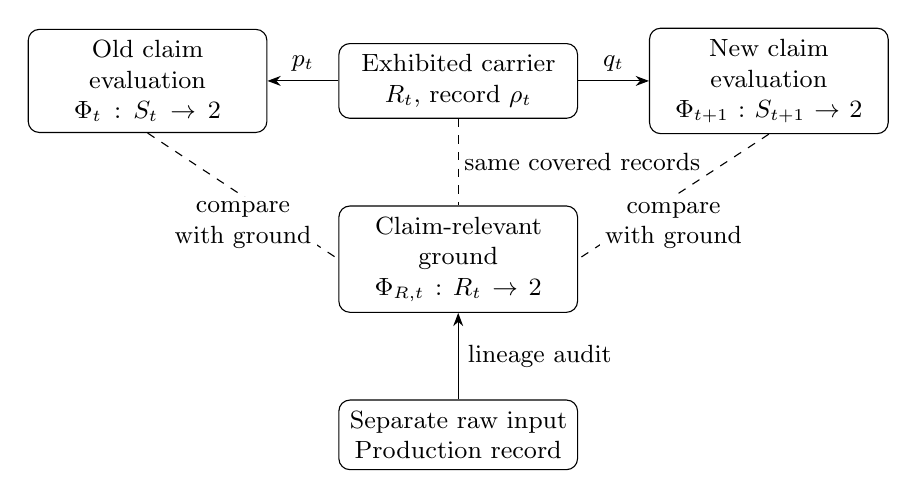
\begin{tikzpicture}[>=Stealth,node distance=1.1cm and 0.9cm,font=\small,
  box/.style={draw,rounded corners,align=center,text width=2.75cm,inner sep=4pt}]
\node[box] (old) {Old claim evaluation\\$\Phi_t:S_t\to2$};
\node[box,right=of old] (carrier) {Exhibited carrier\\$R_t$, record $\rho_t$};
\node[box,right=of carrier] (new) {New claim evaluation\\$\Phi_{t+1}:S_{t+1}\to2$};
\node[box,below=of carrier] (ground) {Claim-relevant ground\\$\Phi_{R,t}:R_t\to2$};
\node[box,below=of ground] (raw) {Separate raw input\\Production record};
\draw[->] (carrier) -- node[above] {$p_t$} (old);
\draw[->] (carrier) -- node[above] {$q_t$} (new);
\draw[->] (raw) -- node[right] {lineage audit} (ground);
\draw[dashed] (carrier) -- node[right,fill=white,inner sep=2pt] {same covered records} (ground);
\draw[dashed] (old.south) -- node[midway,below,fill=white,inner sep=2pt,align=center] {compare\\with ground} (ground.west);
\draw[dashed] (new.south) -- node[midway,below,fill=white,inner sep=2pt,align=center] {compare\\with ground} (ground.east);
\end{tikzpicture}
\caption{Migration audit objects. Each endpoint needs its own observational determination evidence. Dashed links denote evaluation and comparison on the carrier; they are not production edges. Production of the ground is audited separately against (L1)--(L4).}
\label{ex:fig:audit-workflow}
\end{figure}

\begin{definition}[Seam coherence]\label{ex:def:seamcoherence}
The span is seam coherent for $(\Phi_t,\Phi_{t+1})$ when $\Phi_t \circ p_t=\Phi_{t+1} \circ q_t$.
\end{definition}

\paragraph{Engineering reading.} On every covered migrated record, the old and new claim evaluations agree. This is an endpoint-consistency test. It says nothing yet about whether the common value is correct.

\begin{definition}[Seam witness]\label{ex:def:seamwitness}
A seam witness is an element $r \in R_t$ with $\Phi_t(p_t(r)) \neq \Phi_{t+1}(q_t(r))$.
\end{definition}

\paragraph{Engineering reading.} A seam witness is one migrated record on which the old and new evaluations disagree. It is the migration analogue of a failing source--target comparison, but its subject is the declared claim rather than raw row equality.

\begin{proposition}[Span criterion]\label{ex:prop:span}
Suppose the span is seam coherent for $(\Phi_t,\Phi_{t+1})$ and $\Phi_t=\widehat\Phi_t \circ M_t$. Then $\Phi_{t+1} \circ q_t$ factors through $M_t \circ p_t$ as maps on $R_t$.
\end{proposition}

\begin{proof}
By seam coherence and the assumed factorisation,
\[
\Phi_{t+1}\circ q_t=\Phi_t\circ p_t=\widehat\Phi_t\circ M_t\circ p_t,
\]
so $\widehat\Phi_t$ is itself a factor of $\Phi_{t+1}\circ q_t$ through $M_t\circ p_t$.\qed
\end{proof}

Proposition~\ref{ex:prop:span} establishes factorisation on $R_t$ only; it says nothing about states of $S_{t+1}$ outside the image of $q_t$. A changed predicate needs its own certificate. The displayed factor is constructed directly and is used again in the constructive condition on later admissibility.

\subsection{Independent grounding at the seam}\label{ex:sec:grounding-seam}

Extensional seam coherence permits accidental or copied agreement. The engineering question is whether agreement between two coordinate descriptions is supported by a valuation produced from claim-relevant process evidence rather than inherited from either coordinate. Where the process can be exhibited, the assurance record therefore needs a seam valuation with a production path that can be audited independently of the two determinations it is meant to check.

Consider services $A$ and $B$ during a dual-write migration. Service $A$ emits a status line and $B$ copies it into the new-format log. Let $1$ mean ``completed without a partial effect''. On an ordinary request $r_{\mathrm{ok}}$, no partial effect occurs and the trace and both logs correctly support $1$. On request $r_*$, an irreversible side effect occurs before a failure, but $A$ prematurely writes $1$ and $B$ copies it. The execution trace supports $0$:
\[
\Phi_A(p(r_*))
=\Phi_B(q(r_*))=1,
\qquad
\Phi_R(r_*)=0,
\]
where $\Phi_R$ is evaluated from an exhibited trace. Identity evolution makes every update square commute, yet the agreement carries a false claim. Defining $\widetilde\Phi_R=\Phi_A\circ p$ would satisfy the equations only by copying the coordinate. Exhibition instead requires the continuing process, provenance from it to both coordinates, evidence sufficient to evaluate $\Phi_R$, declared coverage, and custody.

Source independence does not exhaust this requirement. Two independently maintained instruments can produce operationally independent reports and still share a blind spot because neither records a process feature on which the claim depends. Such independence may support confidence in the coordinate records without supplying a valuation of the relevant process. Grounded coherence therefore asks a different question: whether the asserted value is exhibited from claim-relevant process occurrences by a production path that runs through neither coordinate.

In the defeater vocabulary of Assurance~2.0 (Section~\ref{ex:sec:related}), a fibre witness defeats the claim that an observation surface determines the predicate; a seam witness defeats extensional transport on the exhibited carrier; a grounding witness defeats the stronger claim that the coordinate values agree with an independent process valuation. Missing carrier or lineage coverage is different again: it undercuts the inference from a clean check, because the relevant case may never have entered the check. The record must therefore exhibit the seam valuation's production path. Conditions (L1)--(L3) below prohibit descent from either coordinate, disclose their shared derived ancestry, and require a claim-relevant raw source outside both coordinate ancestries; Section~\ref{ex:sec:laundering} adds a fourth condition on the ancestry the ground shares with them.

Table~\ref{ex:tab:comparison} separates the claims made by different migration checks; Section~\ref{ex:sec:related} relates them to the testing literature.

\begin{table}[htbp]
\centering\small
\caption{Different claims made by migration checks. A pass in one row does not entail a pass in another.}
\label{ex:tab:comparison}
\begin{tabularx}{\textwidth}{@{}p{2.8cm}LLL@{}}
\toprule
Check & Question & Counterevidence & Positive result needs \\
\midrule
Source--target validation & Does the target match the mapped source? & Unequal mapped records & Declared mapping and checked records \\
Reconciliation & Were the declared source records accounted for? & Missing or duplicated identifiers & Independent totals and stated coverage \\
Seam coherence & Do the two claim valuations agree on the carrier? & One seam witness & Exhibited, sufficiently covered carrier \\
Grounded coherence & Do both valuations agree with a separately produced, claim-relevant seam valuation? & Grounding witness or failed lineage condition & Equations, lineage conditions, and external evidence for carrier and raw-source fidelity \\
\bottomrule
\end{tabularx}
\end{table}

A trace is also a representation. Its claim to ground the seam is defeasible: its documented path must begin in claim-relevant process occurrences and pass through neither coordinate. It may still be inaccurate or incomplete. A copied coordinate cannot establish its own agreement with another coordinate.

Some regimes cannot exhibit an independent ground. The audit then reports incomplete or obstructed lineage, not a grounding witness. If neither a ground nor a refuting witness is available, support for transport is underdetermined. The institution must obtain a new certificate, instrument future transitions, or hold the gap open as debt. It may report coordinate agreement without claiming grounded transport.

Within a migration window, write the concurrent old and new coordinate state models as $A_t$ and $B_t$:
\[
A_t\xleftarrow{p_t}R_t\xrightarrow{q_t}B_t.
\]
The carrier and projections keep the notation introduced above. $A_t$ and $B_t$ name the two schemas at window stage $t$, allowing both to evolve; they replace $S_t$ and $S_{t+1}$ only when the discussion concerns concurrent evolution rather than one consecutive cut-over. Equip $R_t$ with its record and a valuation $\Phi_{R,t}:R_t\to V_t$ from the retained process evidence. The coordinate valuations are $\Phi_{A,t}:A_t\to V_t$ and $\Phi_{B,t}:B_t\to V_t$. For the executable exact claims, $V_t=2$.

The lineage requirement is stated over a declared graph. A \emph{lineage record} for the seam is a finite directed acyclic graph $L$ whose nodes are the fields that enter the three valuations and whose edges run from each field to the fields derived from it. It declares a set $\operatorname{Raw}(L)$ of raw inputs, which enter the regime from outside it and have no incoming edges, and marks the claim-relevant raw inputs $\operatorname{Rel}(L)\subseteq\operatorname{Raw}(L)$. It contains nodes $d_A$, $d_B$, and $g$ for the determinations $\Phi_{A,t}\circ p_t$, $\Phi_{B,t}\circ q_t$, and $\Phi_{R,t}$. Write $\operatorname{anc}(x)$ for the set of strict ancestors of $x$ in $L$.

Figure~\ref{ex:fig:lineage-dag} shows the smallest pattern the three lineage clauses are meant to distinguish. A shared derived node can explain coordinate agreement without corroborating it; a separate raw process source can ground the seam valuation without descending from either coordinate.

\begin{figure}[htbp]
\centering
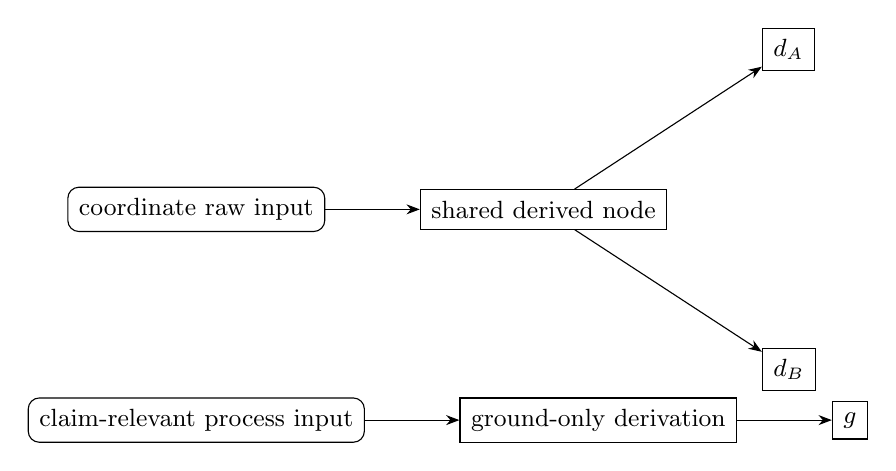
\begin{tikzpicture}[>=Stealth,node distance=1.5cm and 1.2cm,font=\small,
  raw/.style={draw,rounded corners,inner sep=4pt},
  derived/.style={draw,inner sep=4pt}]
\node[raw] (coordraw) {coordinate raw input};
\node[derived, right=of coordraw] (shared) {shared derived node};
\node[derived, above right=of shared] (da) {$d_A$};
\node[derived, below right=of shared] (db) {$d_B$};
\node[raw, below=2.1cm of coordraw] (process) {claim-relevant process input};
\node[derived, right=of process] (groundmid) {ground-only derivation};
\node[derived, right=of groundmid] (g) {$g$};
\draw[->] (coordraw) -- (shared);
\draw[->] (shared) -- (da);
\draw[->] (shared) -- (db);
\draw[->] (process) -- (groundmid);
\draw[->] (groundmid) -- (g);
\end{tikzpicture}
\caption{A lineage pattern with shared coordinate ancestry and a separate claim-relevant ground. The figure is schematic: real records may contain many additional nodes and edges.}
\label{ex:fig:lineage-dag}
\end{figure}

\paragraph{Running-example bridge.} In the tax migration, the backfill route is zone $\to$ primary municipality $\to$ new tax flag. The delivery-based seam valuation instead uses the separately recorded delivery event. The lineage test does not require the new coordinate to be independent of the old one. It requires the \emph{ground used to corroborate them} to have a claim-relevant production path that does not descend from either coordinate, and it makes their shared ancestry explicit.

\begin{definition}[Coordinate-copied ground]\label{ex:def:copied-ground}
A proposed ground node $g$ is \emph{coordinate-copied} relative to $(d_A,d_B)$ when
\[
g=d_A\ \lor\ g=d_B\ \lor\ d_A\in\operatorname{anc}(g)\ \lor\ d_B\in\operatorname{anc}(g).
\]
This is a production-path property, not equality of reported values. Independently produced valuations can coincide without being copies. No coordinate descent (L1) is exactly the negation of this property.
\end{definition}

\begin{definition}[Three-clause lineage qualification]\label{ex:def:lineage-qualified-three}
Let the span with its record $\rho_t$ be exhibited for the claim, and let $L$ be a lineage record for the seam. The valuation $\Phi_{R,t}$ is \emph{lineage-qualified under (L1)--(L3)}, written $\operatorname{LineageQualified}_{123}(\Phi_{R,t};L)$, when
\begin{enumerate}
\item[(L1)] \emph{no coordinate descent}: $g\neq d_A$, $g\neq d_B$, $d_A\notin\operatorname{anc}(g)$, and $d_B\notin\operatorname{anc}(g)$;
\item[(L2)] \emph{shared ancestry disclosure}: the record lists the shared non-raw ancestry $D=(\operatorname{anc}(d_A)\cap\operatorname{anc}(d_B))\setminus\operatorname{Raw}(L)$ and enters each element of $D$ either with a justification or as an open defeater to inference from coordinate agreement;
\item[(L3)] \emph{independent raw source}: the ground-only source set
\[
G=\bigl(\operatorname{anc}(g)\cup\{g\}\bigr)\setminus
\bigl(\operatorname{anc}(d_A)\cup\operatorname{anc}(d_B)\cup\{d_A,d_B\}\bigr)
\]
contains at least one claim-relevant raw input: $G\cap\operatorname{Rel}(L)\neq\emptyset$.
\end{enumerate}
\end{definition}

\paragraph{Engineering reading of (L1)--(L3).} (L1) says that the corroborating ground must be neither the old nor the new determination, nor derived from either. It is a condition on the ground, not a prohibition on the target field being copied during a migration. (L2) says to list shared derived dependencies of the two coordinates, such as a common zone lookup or upstream service, and record whether each dependency has been answered or remains an open defeater. (L3) says that the ground must have at least one claim-relevant raw source outside both coordinate ancestries. In the running example the delivery event plays that role. A new municipality backfilled from the old zone can therefore be audited, but it cannot serve as its own corroboration.

\paragraph{A three-source example.} Let a raw address $a$ produce a derived zone $z$, with $z\to d_A$ and $z\to d_B$, while a separate claim-relevant raw delivery event $h$ produces $g$. Then no coordinate descends into $g$, so (L1) passes. The shared non-raw ancestor set is $D=\{z\}$, so (L2) requires a disposition for $z$. The event $h$ is outside both coordinate ancestries and witnesses (L3). Leaving $z$ as an open defeater satisfies disclosure without resolving the concern. Replacing the delivery-based ground by $d_A\to g$ makes it coordinate-copied and fails (L1), even if its numerical output remains unchanged.

Claim relevance is a declaration attached to a raw input for the specified claim. The structural audit checks that the input is declared, raw, consistently marked, and in the required ground-only set. It does not prove that the marking is true or that the instrument captured the relevant occurrence faithfully.

The clauses prevent three different errors, and each can fail while the other two hold. Since ancestry is strict, the explicit inequalities in (L1) exclude the degenerate case in which the purported ground is a coordinate node itself. The absence of each coordinate from $\operatorname{anc}(g)$ excludes any directed dependency path from that coordinate to the ground. (L2) exposes shared derived ancestry that could explain agreement without corroboration. The inclusion of $g$ in (L3) permits a direct raw process input to serve as the ground; its exclusion from both coordinate ancestries still has to be checked. A claim-relevant raw input on the ground's route alone is a necessary graph condition, not proof that the recorded route exhausts the actual production of the valuation.

\paragraph{Current executable criterion.} The current artefact reflects (L1)--(L4), with (L4) as defined in Section~\ref{ex:sec:laundering}, for finite declared records with derived coordinates and a raw or derived ground. Appendix~\ref{ex:app:verification} gives the claim-to-proof map, runtime boundary, and reproduction sequence.

\paragraph{Structural passing and certificate issuance.}
Conditions (L2) and (L4) are disclosure conditions. Recording a shared ancestor as an open defeater satisfies disclosure but does not discharge the concern. A structural pass under (L1)--(L4) therefore does not license an unqualified transport certificate. Issuance also requires every declared defeater to be resolved, no outstanding coverage gaps, and the remaining transport obligations. Keeping these requirements separate from (L2) and (L4) preserves the difference between an accurate record of a concern and evidence that answers it.

\paragraph{Adversarial and incomplete records.} The custodian of Definition~\ref{ex:def:exhibited-seam} holds $L$. Passing (L1)--(L4) checks the declared derivation, not the graph's completeness or the raw source's accuracy, and an omitted production path may defeat the assurance (Section~\ref{ex:sec:case-audit}). A fabricated graph can satisfy the syntax while misdescribing production, and a materially incomplete one can hide descent from a coordinate. The threats are concrete: an operator may omit failed writes to meet a cut-over target, a backfill service may label a copied zone lookup as geocoded, a compromised producer may emit false source events, or a later custodian may remove a dependency that reveals copying. Distinct controls address distinct opportunities. Binding lineage records to source and deployment identifiers and reconciling declared paths against independently held totals challenge omission. Authenticated, tamper-evident event capture makes later alteration detectable, although it cannot show that the history was complete or truthful when created. Independent validation of a sample challenges a false value at capture. The assurance record should name the producer of each lineage edge, the retention and access controls, and any portion for which independent corroboration is unavailable.

\paragraph{Binding is necessary but not grounding.}
A certificate, proposal, or migration record can be internally valid and still be attached to the wrong assertion. A transport record should therefore bind the claim, the old and new versions, the computed coordinate statuses, the seam record, and the lineage result that is asserted about them. Where possible, the downstream record should be constructed from those actual objects rather than accept a caller-supplied certificate whose subject is merely assumed to match. This prevents one claim's warrant record from being substituted for another, but it does not establish an independent ground: a perfectly bound certificate can still certify a value copied from one coordinate, and two correctly bound records can still share one production source.

The graph need not be stored in the paper's bespoke notation. A deployment can encode raw observations and derived records as PROV entities, transformations as activities, and responsible services or people as agents \citep{w3cprovdm2013}; derivation edges then supply the ancestry relation used by the audit. PROV records a declared history; it does not by itself guarantee that the history is complete, that a source is claim-relevant, or that two records are independent in the sense required here.

For relational queries, provenance-semiring annotations can preserve alternatives and joint dependencies that a simple edge list may flatten \citep{greenkarvounarakistannen2007}. Conditions (L1)--(L4) apply to them only after an explicit account maps annotations and transformation steps to the distinguished valuations and declares the relevant raw sources; the occurrence of a coordinate variable in one derivation differs from its being a factor of every derivation. No such mapping is implemented here.

A partial lineage record can support only a coverage-qualified result. The record must mark the nodes, transformations, versions, and transition interval it covers. Any unrecorded claim-relevant segment remains an open construction obligation, and the audit reports ``pass relative to $L$'' together with the gap, not global lineage grounding. Where several candidate grounds $g_1,\ldots,g_k$ exist, each candidate is audited separately against (L1)--(L4) and its own coverage. One candidate suffices only for the seam elements and claim for which it is exhibited and claim-relevant. Combining partial grounds requires an explicit aggregation map and a coverage argument; distinct field names do not establish independence, and shared ancestry among the grounds must itself be declared. If no candidate covers the asserted transition, transport remains underdetermined even when every audited fragment passes.

For an incomplete legacy source, the custodian inventories the surviving schemas, writes, versions, and independent traces, marking the interval and claims each covers. A reconstructed path is entered as an inference, never as a raw observation. The audit returns a counterexample, a pass relative to a bounded graph, or an obstruction of the required history. The institution must then narrow the transport claim, obtain new evidence, or operate with marked debt. Obstruction establishes no fact about the missing path.

\subsection{Grounds that launder shared ancestry}\label{ex:sec:laundering}

Condition (L1) forbids the ground from descending from the coordinate determinations, but not from their ancestors. A ground can therefore pass (L1)--(L3) while reading a derived node that also feeds both coordinates.

\begin{proposition}[Laundering through shared ancestry]\label{ex:prop:laundering}
There is an exhibited seam with a lineage record satisfying (L1)--(L3) whose seam valuation is a function of a derived node shared by both coordinates, satisfies both grounding equations, and is false at a seam record.
\end{proposition}
\begin{proof}
Use the dual-write services example of Section~\ref{ex:sec:grounding-seam}: the carrier $R=\{r_{\mathrm{ok}},r_*\}$ is exhibited by the two request identifiers, their old and new log entries, the execution trace, coverage $C=R$, and a declared custodian; both coordinate valuations equal $1$ at both records; and the trace records a partial effect at $r_*$. Take raw nodes $a,h$, derived nodes $s,d_A,d_B,g$, and the edges
\[
a\to s,\qquad s\to d_A,\qquad s\to d_B,\qquad s\to g,\qquad h\to g,
\]
with $s$ the shared status line, $h$ the trace, and $\operatorname{Rel}(L)=\{h\}$. Then $\operatorname{anc}(g)=\{a,s,h\}$ contains neither coordinate, and $g$ differs from both, so (L1) holds. The shared non-raw coordinate ancestry is $D=\{s\}$, which can be disclosed, so (L2) holds. The ground-only set is $\{h,g\}$, which contains the claim-relevant $h$, so (L3) holds. Let the seam valuation be the recorded status line, $\Phi_R(r)=v_s(r)$, which is $1$ at both records. Both grounding equations $\Phi_A\circ p=\Phi_R=\Phi_B\circ q$ hold, yet the trace shows that the claim fails at $r_*$.\qed
\end{proof}

The proposition exposes two gaps at once. (L1) does not look upstream of the coordinates, and (L3) asks only that a claim-relevant source be present in the ground's ancestry, not that the valuation use it. Here $h$ is present and ignored.

\begin{definition}[Ground-ancestry disclosure and strict separation]\label{ex:def:separation}
For a lineage record $L$ with distinguished nodes $d_A,d_B,g$, let
\[
E_g=\bigl(\operatorname{anc}(g)\cap(\operatorname{anc}(d_A)\cup\operatorname{anc}(d_B))\bigr)\setminus\operatorname{Raw}(L)
\]
be the derived ancestry that the ground shares with either coordinate. The record satisfies
\begin{enumerate}
\item[(L4)] \emph{ground-ancestry disclosure} when it lists $E_g$ and enters each element either with a justification or as an open defeater to inference from agreement with the ground.
\end{enumerate}
The ground is \emph{strictly separated} when $E_g=\emptyset$. Condition (L4) establishes disclosure and inspectability; it does not establish separation when shared derived dependencies remain.
\end{definition}

\begin{definition}[Lineage qualification and clearance]\label{ex:def:lineage-qualified}
An exhibited seam valuation is \emph{lineage-qualified} by $L$, written $\operatorname{LineageQualified}(\Phi_{R,t};L)$, when $\operatorname{LineageQualified}_{123}(\Phi_{R,t};L)$ and (L4) hold. This is the structural (L1)--(L4) status. It can hold with disclosed defeaters still open.

For a declared claim and scope $C$, it is \emph{lineage-cleared}, written
\[
\operatorname{LineageCleared}(\Phi_{R,t};L,C),
\]
when it is lineage-qualified, evidence resolves the declared lineage defeaters, no claim-relevant lineage-coverage gap remains within $C$, and an evaluator-adequacy justification establishes how its computation evaluates the declared claim from the relevant evidence on that scope. Clearance is an assurance judgement recorded for that claim and scope. The graph check alone does not establish clearance, evaluator adequacy, raw-source fidelity, or any of the remaining transport obligations. A faithful raw source can be present in the graph and ignored by the evaluator; fidelity and substantive use therefore need separate evidence.
\end{definition}

(L4) permits the ground to share raw inputs with the coordinates, such as a charged rate or a published rate table, which a valuation of the same claim will often need. It requires every shared \emph{derived} input to be named. Like (L2), it is a disclosure condition: an open (L4) defeater satisfies the structural condition and blocks issuance. In Proposition~\ref{ex:prop:laundering}, $E_g=\{s\}$, so the laundered ground passes (L4) only by recording the status line as an open defeater or by justifying it.

Where a justification asserts that retained shared ancestry does not determine the ground, the fibre criterion supplies a finite test of that extensional assertion. Suppose the record retains, for each seam element $r$, the tuple $v_E(r)$ of values recorded at the nodes of $E_g$.

\begin{proposition}[A fibre test for laundering]\label{ex:prop:laundering-test}
$\Phi_{R,t}$ is $v_E$-admissible on $R_t$ if and only if there is no pair $r,r'\in R_t$ with $v_E(r)=v_E(r')$ and $\Phi_{R,t}(r)\neq\Phi_{R,t}(r')$.
\end{proposition}
\begin{proof}
Lemma~\ref{ex:prop:fibre}, in its nonempty-codomain form, with $R_t$ for $S$, $v_E$ for $M$, and $\Phi_{R,t}$ for $\Phi$.\qed
\end{proof}

If the ground is $v_E$-admissible, its retained values factor through the retained shared-ancestry values on the exhibited carrier. This is an extensional result on those records, not an account of how the ground was produced. A clean test supplies no separation witness, so a nonempty shared-ancestry concern stays open unless other evidence answers it. A witness pair shows that the retained ground distinguishes records that the retained shared ancestry identifies. It refutes the factorisation but does not prove causal independence, substantive use of the (L3) source, or that source's fidelity. Conversely, a genuinely independent ground can factor through the shared values by coincidence on a restricted carrier, so a clean test does not prove copying. In Proposition~\ref{ex:prop:laundering}, the laundered valuation $\Phi_R=v_s$ is trivially $v_s$-admissible. Had the trace valuation been recorded with the same edge $s\to g$, the pair $(r_{\mathrm{ok}},r_*)$, which agrees on the status line and differs on the trace, would refute $v_s$-admissibility. On a finite carrier the test is the reference procedure of Section~\ref{ex:sec:finite-procedure} with $v_E$ as the observation map. If the record does not retain the values of the shared nodes, the defeater cannot be resolved this way and remains open.

\begin{proposition}[Injective tuples make the fibre test nondiscriminating]\label{ex:prop:injective-tuple}
If $v_E:R_t\to O$ is injective, every Boolean valuation $\Phi_{R,t}$ is $v_E$-admissible on $R_t$.
\end{proposition}
\begin{proof}
Equality of tuples implies equality of carrier records, hence equality of their valuations. Apply the fibre criterion. For an executable positive result on a finite carrier, complete enumeration is still required.\qed
\end{proof}

\paragraph{Diagnostic scope of the tuple.} A retained shared record identifier can make the tuple injective. The test then cannot produce a separation witness, however independently the ground was produced; a factor table does not establish copying. Each diagnostic run must identify the dependency it investigates, the tuple components it uses, and whether they distinguish every carrier record. If a narrower dependency $F\subseteq E_g$ is tested, the result concerns $v_F$, not automatically $v_E$; adding an identifier can destroy the collisions needed for a witness. The full (L4) disclosure obligation remains unchanged.

\begin{proposition}[Shared raw inputs can leave an independent source unused]\label{ex:prop:raw-ignored-source}
There is an acyclic declared graph satisfying (L1)--(L4), with $E_g=\emptyset$, whose proposed ground ignores the claim-relevant independent raw source and agrees with both coordinates while contradicting that faithful source on one carrier record.
\end{proposition}
\begin{proof}
Take raw inputs $a,h$, derived nodes $d_A,d_B,g$, and exactly the edges
\[
a\to d_A,\qquad a\to d_B,\qquad a\to g,\qquad h\to g,
\]
with $\operatorname{Rel}(L)=\{h\}$. The ground is distinct from and descends from neither coordinate, so (L1) holds. All shared ancestry is raw, so (L2) and (L4) are vacuous and $E_g=\emptyset$. The ground-only source set contains $h$, witnessing (L3). On $R=\{r_{\mathrm{ok}},r_*\}$ let $v_a=(1,1)$ and the faithful claim evidence $v_h=(1,0)$. Let both coordinate determinations and the proposed ground return $v_a$, ignoring $h$. Both grounding equations hold, but the proposed ground is wrong at $r_*$. The declared graph records availability of $h$, not substantive dependence of the evaluator on it.\qed
\end{proof}

This is a remaining assurance boundary, not a failure of the graph reflection theorem. Even strict separation excludes only shared \emph{derived} ancestry. Evaluator adequacy must therefore be justified directly; it cannot be inferred from source fidelity, ancestry membership, or agreement.

\subsection{Grounded seam coherence}\label{ex:sec:grounded-coherence}

\begin{definition}[Grounded seam coherence]\label{ex:def:grounded-seam}
Let $A_t \xleftarrow{p_t} R_t
\xrightarrow{q_t} B_t$ be a seam, with valuations
$\Phi_{A,t}:A_t\to V_t$, $\Phi_{B,t}:B_t\to V_t$, and
$\Phi_{R,t}:R_t\to V_t$. The seam is \emph{groundedly coherent} when (a) the span with its record $\rho_t$ is exhibited for the claim (Definition~\ref{ex:def:exhibited-seam}); (b) the record contains a lineage record $L$ by which $\Phi_{R,t}$ is lineage-qualified under (L1)--(L4) (Definition~\ref{ex:def:lineage-qualified}); and (c) the grounding equations hold:
\[
\Phi_{A,t}\circ p_t
=\Phi_{R,t}
=\Phi_{B,t}\circ q_t.
\]
Equivalently, for every $r\in R_t$,
\[
\Phi_{A,t}(p_t(r))
=\Phi_{R,t}(r)
=\Phi_{B,t}(q_t(r)).
\]
\end{definition}

\paragraph{Engineering reading.} A structural grounded-coherence pass requires an auditable migration population, a claim-relevant valuation with lineage qualification, and equality of both coordinate evaluations with that valuation on every covered record. Any disclosed defeater remains open until clearance is separately recorded. Matching old and new outputs establishes only that the coordinates agree with each other.

\begin{table}[htbp]
\centering\small
\caption{Levels of a migration claim. Every result retains its declared claim and coverage.}
\label{ex:tab:claim-levels}
\begin{tabularx}{\textwidth}{@{}p{3.1cm}LL@{}}
\toprule
Status & Formal obligation & Record and institutional obligation \\
\midrule
Lineage-qualified & (L1)--(L4) pass on the declared graph & Exhibited valuation and source declarations; open (L2) and (L4) defeaters remain open \\
Lineage-cleared & Lineage-qualified & Declared lineage defeaters resolved and lineage coverage closed for the claim and scope; source fidelity remains a premise \\
Groundedly coherent & Lineage-qualified ground and both grounding equations & Exhibited span and record; carrier and source fidelity remain stated premises \\
Structurally transportable & Grounded coherence, inhabited carrier, endpoint admissibility, functorial evolution & Evidence bound to the same claim and declared interval \\
Transportable for issuance & All structural obligations established & Declared defeaters and coverage gaps resolved; maintained evidence and authorised custody for the claim and use \\
\bottomrule
\end{tabularx}
\end{table}

Grounded coherence is structural: it can coexist with an unresolved disclosed lineage concern. It implies coordinate agreement. The converse fails: a valuation copied from one coordinate can satisfy the equations while failing lineage condition (b). The extra structure makes the proposed ground inspectable; it does not establish that the carrier adequately represents the process.

\begin{proposition}[Grounding entails extensional seam coherence]\label{ex:prop:grounding-entails-coherence}
Every groundedly coherent seam is seam coherent in the sense of Definition~\ref{ex:def:seamcoherence}.
\end{proposition}

\begin{proof}
For every $r\in R_t$, both
$\Phi_{A,t}(p_t(r))$ and
$\Phi_{B,t}(q_t(r))$ are equal to
$\Phi_{R,t}(r)$.\qed
\end{proof}

\begin{definition}[Grounding witness]\label{ex:def:grounding-witness}
A grounding witness for a seam with an exhibited, lineage-qualified valuation $\Phi_{R,t}$ is an element $r\in R_t$ with $\Phi_{A,t}(p_t(r))\neq\Phi_{R,t}(r)$ or $\Phi_{B,t}(q_t(r))\neq\Phi_{R,t}(r)$.
\end{definition}

\paragraph{Engineering reading.} This is the row that an endpoint comparison can miss. At least one endpoint disagrees with the separately produced ground, although the two endpoints may still agree with each other. The running row $(2,5,\mathit{general},\mathit{before},60)$ is exactly that case: the copied flags agree, while the delivery-based valuation disagrees.

Read on the carrier $R_t$, every seam witness in the sense of Definition~\ref{ex:def:seamwitness} is a grounding witness, because two coordinate values that differ cannot both equal $\Phi_{R,t}(r)$. The converse fails, and that failure is the point of the grounded condition. A single grounding witness refutes grounded coherence, as a single seam witness refutes extensional coherence; the checked lemmas are identified in Appendix~\ref{ex:app:verification}.

\begin{proposition}[Ungrounded agreement]\label{ex:prop:ungrounded-agreement}
There exist exhibited spans whose coordinate predicates satisfy extensional seam coherence and whose identity update maps satisfy functorial commutation, but for which grounded coherence fails: the lineage-qualified process valuation disagrees with both coordinates, and the valuation that agrees with them fails the lineage condition. Such a span can transport a false claim.
\end{proposition}

\begin{proof}
Let $R=\{r_{\mathrm{ok}},r_*\}$, $A=\{a_{\mathrm{ok}},a_*\}$, and $B=\{b_{\mathrm{ok}},b_*\}$. Define $p(r_i)=a_i$ and $q(r_i)=b_i$, and let both coordinate predicates be constantly $1$. Thus $\Phi_A\circ p=\Phi_B\circ q$ on all of $R$. Repeat these sets and maps at every stage and take all update maps to be identities. Both naturality squares, the identity laws, and the composition laws then hold directly. Identity evolution makes these checks vacuous with respect to change; it supplies no grounding evidence.

Exhibit the two request identifiers, their old and new log entries, the execution trace, coverage $C=R$, and a declared custodian in $\rho$. The trace valuation is $\Phi_R(r_{\mathrm{ok}})=1$ and $\Phi_R(r_*)=0$: at $r_*$ it records the partial effect missed by the status line. These declarations satisfy the five exhibition conditions in this finite countermodel.

For lineage, take raw nodes $a,h$, derived nodes $s,d_A,d_B,g$, and exactly the edges
\[
a\to s,\qquad s\to d_A,\qquad s\to d_B,\qquad h\to g.
\]
Here $s$ is the shared status line, $h$ is the claim-relevant trace, and $\operatorname{Rel}(L)=\{h\}$. The graph is acyclic. Its strict ancestor sets are
\[
\operatorname{anc}(d_A)=\operatorname{anc}(d_B)=\{a,s\},
\qquad \operatorname{anc}(g)=\{h\}.
\]
The three distinguished nodes are distinct, and neither coordinate is an ancestor of $g$, so (L1) holds. The shared non-raw set is $D=\{s\}$; disclosing $s$ as an open defeater satisfies (L2). The ground-only set is $G=\{h,g\}$, so $G\cap\operatorname{Rel}(L)=\{h\}$ and (L3) holds. Since $\operatorname{anc}(g)=\{h\}$ shares nothing with the coordinates, $E_g=\emptyset$ and the ground is strictly separated. This proves lineage qualification without an executable audit. At $r_*$, however, both coordinate values are $1$ and $\Phi_R(r_*)=0$. The grounding equations fail, so grounded coherence fails despite endpoint equality and functorial commutation.

For the agreeing alternative, add a fresh node $\widetilde g$ with the single incoming edge $d_A\to\widetilde g$ and valuation $\widetilde\Phi_R=\Phi_A\circ p$. It is constantly $1$, so both grounding equations hold. But $d_A\in\operatorname{anc}(\widetilde g)$, violating (L1). Also
\[
\operatorname{anc}(\widetilde g)=\{a,s,d_A\},
\qquad \widetilde G=\{\widetilde g\},
\]
and $\widetilde G\cap\operatorname{Rel}(L)=\emptyset$, violating (L3). Thus the valuation that matches the endpoints is coordinate-copied, while the lineage-qualified valuation refutes their common claim. The record $r_*$ is a grounding witness and is not a seam witness.\qed
\end{proof}

The Coq development checks the equational part through \code{copied\_\allowbreak not\_\allowbreak grounded} and \code{grounding\_\allowbreak witness\_\allowbreak refutes}. The current executable audit checks the corresponding declared lineage cases; the paper proof does not depend on executing them.

\begin{proposition}[Claim-specific admissibility can pass before grounding fails]\label{ex:prop:claim-control}
Both endpoint observation surfaces can determine the actual claim $\chi$ while their implemented outputs agree and the grounding equations fail.
\end{proposition}
\begin{proof}
Use a two-record carrier and corresponding two-state endpoints with identity projections and observation maps. On each endpoint let the actual claim be $\chi=(1,0)$. It factors through the identity observation by taking $\chi$ itself as factor. Let both implemented endpoint predicates return $(1,1)$ and the independent trace ground return $\chi=(1,0)$. Endpoint outputs agree on both records, but the grounding equations fail on the second. The ground can have the strictly separated trace lineage in Proposition~\ref{ex:prop:ungrounded-agreement}. Both claim-specific admissibility conjuncts pass; implementation correctness and grounded coherence do not.\qed
\end{proof}

\begin{table}[htbp]
\centering\small
\caption{Two-record control for the actual claim; determination does not certify the implementation.}\label{ex:tab:claim-control}
\begin{tabularx}{\textwidth}{@{}lL@{}}
\toprule
Check & Result \\
\midrule
Old surface determines $\chi$ & Pass: identity observation, $\chi=(1,0)$ \\
New surface determines $\chi$ & Pass: identity observation, $\chi=(1,0)$ \\
Implemented outputs agree & Pass: both return $(1,1)$ \\
Independent ground evaluates $\chi$ & Trace valuation $(1,0)$ \\
Grounding equations & Fail at the second record \\
\bottomrule
\end{tabularx}
\end{table}

The practical consequence is that the assurance record must contain the ground, its production path and evaluator justification, not only the two coordinate values.

\section{Evolution and composition}\label{ex:sec:evolution}

\subsection{Functorial transport}\label{ex:sec:functorial-transport}

This subsection asks whether multi-stage updates preserve the record relationships when the seam and both coordinates evolve. Checking one cut-over pair is not enough if a longer migration is certified by composing several stages.

Grounding at one stage does not constrain evolution. For stages $t\leq u$, let the seam and its coordinates evolve from $t$ to $u$ by
$U^{R}_{t,u}:R_t\to R_u$, $U^{A}_{t,u}:A_t\to A_u$, and $U^{B}_{t,u}:B_t\to B_u$. The persistence of the seam process must determine the persistence of its coordinate descriptions, which requires the squares
\begin{equation}\label{ex:eq:dynamic-squares}
\begin{tikzcd}[column sep=large,row sep=large,baseline=(current bounding box.center)]
R_t \arrow[r,"U^{R}_{t,u}"] \arrow[d,"p_t"']
  & R_u \arrow[d,"p_u"] \\
A_t \arrow[r,"U^{A}_{t,u}"'] & A_u
\end{tikzcd}
\qquad
\begin{tikzcd}[column sep=large,row sep=large,baseline=(current bounding box.center)]
R_t \arrow[r,"U^{R}_{t,u}"] \arrow[d,"q_t"']
  & R_u \arrow[d,"q_u"] \\
B_t \arrow[r,"U^{B}_{t,u}"'] & B_u
\end{tikzcd}
\end{equation}
to commute:
\begin{align}
p_{u}\circ U^R_{t,u} &=U^A_{t,u}\circ p_{t},\label{ex:eq:back-naturality}\\
q_{u}\circ U^R_{t,u} &=U^B_{t,u}\circ q_{t}. \label{ex:eq:fwd-naturality}
\end{align}
These are naturality conditions: the projections are natural transformations from the seam evolution to the coordinate evolutions. Their content is that a process cannot acquire incompatible histories because two architectural descriptions were evolved independently. The evolution maps must also satisfy, for $X \in \{R,A,B\}$ and stages $t\leq u\leq v$,
\begin{align}
U^{X}_{t,t} &=\operatorname{id}_{X_t},\label{ex:eq:evolution-identity}\\
U^{X}_{t,v} &=U^{X}_{u,v}\circ U^{X}_{t,u},\label{ex:eq:evolution-composition}
\end{align}
so that each assignment $t \mapsto X_t$, $(t\leq u)\mapsto U^X_{t,u}$ is a functor from the ordered set $(T,\leq)$, regarded as a category, to the category of sets. Without Equation~\eqref{ex:eq:evolution-composition}, the map used for a long migration could differ from the composite of its certified parts.

\begin{proposition}[Commutation composes]\label{ex:prop:commutation-composes}
If the squares commute for $t\to u$ and $u\to v$, and Equations~\eqref{ex:eq:evolution-identity} and~\eqref{ex:eq:evolution-composition} hold, the squares commute for $t\to v$.
\end{proposition}

\begin{proof}
For every $r \in R_t$,
\begin{align*}
p_v(U^R_{t,v}(r))
&=p_v(U^R_{u,v}(U^R_{t,u}(r)))
=U^A_{u,v}(p_u(U^R_{t,u}(r)))\\
&=U^A_{u,v}(U^A_{t,u}(p_t(r)))
=U^A_{t,v}(p_t(r)).
\end{align*}
The forward case replaces $A$ and $p$ by $B$ and $q$.\qed
\end{proof}

Grounded coherence is synchronic and functorial commutation is diachronic. Neither requires the valuation to stay unchanged. If the value spaces carry a transport $U^V_{t,u}$, one may add $\Phi_{R,u} \circ U^R_{t,u}=U^V_{t,u} \circ \Phi_{R,t}$; without such a transport, requiring $\Phi_{R,u} \circ U^R_{t,u}=\Phi_{R,t}$ would turn a dynamic predicate into a temporal invariant.

\paragraph{Claims and their implementations.} The transport definition below needs one more distinction. Let $\chi$ be the declared claim of Definition~\ref{ex:def:coverage}, and write $\chi_t:S_t\to2$ and $\chi_{t+1}:S_{t+1}\to2$ for its evaluation on the two stage models. That each stage model represents the claim-relevant occurrence is a relevance obligation. The coordinate predicates $\Phi_t$ and $\Phi_{t+1}$ are the institution's implementations of $\chi$, and the seam valuation $\Phi_{R,t}$ evaluates $\chi$ from process evidence. In the cut-over reading $A_t=S_t$ and $B_t=S_{t+1}$, so that $\Phi_{A,t}=\Phi_t$ and $\Phi_{B,t}=\Phi_{t+1}$. A certificate that $\Phi_t$ is admissible on $M_t$ is a fact about $\Phi_t$. It bears on $\chi$ only where $\Phi_t=\chi_t$ on the certified scope; otherwise it certifies a different claim, and the gap is a relevance defect rather than an admissibility pass. The endpoint conjuncts of transport are therefore stated for $\chi$.

\begin{definition}[Structural transport and certificate issuance]\label{ex:def:nonvacuous-transport}
The claim $\chi$ is structurally transportable from $t$ to $t+1$ over the declared interval when
\[
\begin{aligned}
\operatorname{StructuralTransport}_{t,t+1} \Longleftrightarrow{}&
\operatorname{Inhabited}(R_t) \land \operatorname{Exhibited}(\rho_t) \\
&{}\land \operatorname{LineageQualified}(\Phi_{R,t};L_t) \\
&{}\land \operatorname{Admissible}_{M_t}(\chi_t) \land \operatorname{Admissible}_{M_{t+1}}(\chi_{t+1}) \\
&{}\land \operatorname{GroundingEquations}_t \land \operatorname{Functorial}(U;I_t).
\end{aligned}
\]
Certificate issuance additionally requires
\[
\begin{aligned}
\operatorname{Transportable}_{t,t+1}(C)\Longleftrightarrow{}&
\operatorname{StructuralTransport}_{t,t+1}\\
&{}\land\operatorname{DefeatersResolved}(\rho_t,L_t;C)\\
&{}\land\operatorname{CoverageClosed}(\rho_t,L_t;C)\\
&{}\land\operatorname{CurrentEvidenceAndCustody}(\rho_t;C).
\end{aligned}
\]
The latter predicates name assurance obligations recorded for the claim, use, time, and scope $C$, including evaluator adequacy within defeater resolution and the ground's construction warrant; they are not new mechanically proved properties of the concrete process.
\end{definition}

Here $R_t$ is the carrier of the span exhibited by $\rho_t$, $L_t$ is its lineage record, and the grounding-equation conjunct is the pair of equations in condition (c) of Definition~\ref{ex:def:grounded-seam}. The exhibition, lineage qualification, and equation conjuncts are conditions (a), (b), and (c) of that definition, listed separately so that each can be assessed and reported on its own; together they are grounded coherence. The Coq development uses the same name for the equational conjunct alone. The functoriality conjunct is a property of the whole family of evolution maps $U=\{U^X_{u,v}\mid X\in\{R,A,B\},\ u\leq v,\ u,v\in I_t\}$ over the declared interval $I_t\subseteq T$, not of a single transition. It requires every naturality square in Equations~\eqref{ex:eq:back-naturality} and~\eqref{ex:eq:fwd-naturality} to commute, and Equations~\eqref{ex:eq:evolution-identity} and~\eqref{ex:eq:evolution-composition} to hold, for all composable stages in $I_t$.

Section~\ref{ex:sec:pcfw} states how checked endpoint evidence may discharge the observational conjuncts; the remaining conjuncts need their own evidence. Read operationally, the definition is a sequence rather than an opaque conjunction: confirm that some process element crosses the interval, exhibit the carrier and its coverage, audit the lineage of the proposed ground, establish admissibility at both endpoints, test the grounding equations on the seam, and check naturality, identity, and composition over the declared interval. A failure stops the transport claim at that stage; later checks may still be diagnostically useful, but they do not repair the failed obligation.

An empty seam satisfies the universal equations vacuously and transports nothing; if no process continues through the interval, any later assertion requires a new certificate. A seam whose carrier and projections are not exhibited has not had its coherence disproved, but that coherence is unauditable and supplies no warrant. If the observation surface itself changes from $O_t$ to $O_{t+1}$ and coherence is asserted at the observational level, an explicit translation between surfaces is also required (Section~\ref{ex:sec:debt-extensions}). The obligation is not specific to software: wherever separately updated coordinate models describe one declared process, the same squares state what it means for them to remain its projections.

\emph{DefeatersResolved} requires evidence answering each declared open concern rather than merely recording it. \emph{CoverageClosed} requires evidence or an explicit narrowing of $C$ for outstanding carrier and lineage gaps within the assertion's scope. \emph{CurrentEvidenceAndCustody} records continued adequacy, evidence retention, and authorised responsibility. Each may be inspected or challenged; none is established by the structural conjunction alone.

The claim that an audit covered a transition needs an assurance procedure outside the checker. Three completeness questions remain separate: whether the state model contains the distinctions relevant to the claim, whether the seam carrier covers the asserted interval, and whether the lineage record captures the production paths actually used. Section~\ref{ex:sec:practice} lists what a carrier declaration should contain, and the custodian should reconcile its counts against independent source totals where available. Sampling and reconciliation can expose omissions but cannot prove an unreachable remainder complete. An adjudicator need not replay a Coq proof to challenge coverage. They need the signed carrier declaration, a readable account of how records entered it, a comparison with independently held totals or samples, and a route to demand missing categories.

\subsection{Composition of seams}\label{ex:sec:lineage-composition}

A long migration is often certified step by step. Proposition~\ref{ex:prop:commutation-composes} shows that commutation composes; this subsection asks the same question of grounding. Let consecutive seams $A_0\xleftarrow{p_{01}}R_{01}\xrightarrow{q_{01}}A_1$ and $A_1\xleftarrow{p_{12}}R_{12}\xrightarrow{q_{12}}A_2$ share the middle coordinate, and form the composite carrier
\[
R_{02}=R_{01}\times_{A_1}R_{12}=\{(r,r')\in R_{01}\times R_{12}\mid q_{01}(r)=p_{12}(r')\},
\]
with projections $p_{02}(r,r')=p_{01}(r)$ and $q_{02}(r,r')=q_{12}(r')$.

\begin{proposition}[Grounding equations compose]\label{ex:prop:equations-compose}
Let $\Phi_i:A_i\to V$ for $i=0,1,2$, and suppose both seams satisfy their grounding equations with the same middle valuation $\Phi_1$. Then $\Phi_{R,01}(r)=\Phi_{R,12}(r')$ for every $(r,r')\in R_{02}$, and $\Phi_{R,02}(r,r')=\Phi_{R,01}(r)$ satisfies $\Phi_0\circ p_{02}=\Phi_{R,02}=\Phi_2\circ q_{02}$.
\end{proposition}
\begin{proof}
For $(r,r')\in R_{02}$,
\[
\begin{aligned}
\Phi_0(p_{01}(r))&=\Phi_{R,01}(r)=\Phi_1(q_{01}(r))\\
&=\Phi_1(p_{12}(r'))=\Phi_{R,12}(r')=\Phi_2(q_{12}(r')).\qquad\qed
\end{aligned}
\]
\end{proof}

The composite carrier still needs its own exhibition record: identifiers for the paired records, provenance through the middle coordinate, and a coverage declaration for the composite interval. The lineage conditions need a separate analysis. The results below fix one ground node $g$ and coordinate nodes $d_0,d_1,d_2$ in one acyclic lineage graph, and write $D_{ij}$, $G_{ij}$, and $E^{ij}_g$ for the sets of Definitions~\ref{ex:def:lineage-qualified-three} and~\ref{ex:def:separation} computed for the pair $(d_i,d_j)$.

\paragraph{What a fixed ground means operationally.}
The shared node $g$ must be stably bound to the same claim, valuation semantics, production source or explicitly identified source family, and the coverage relevant to the composed interval. The common lineage graph must retain the versions of the paths used at both steps. On paired records, the local ground evaluations must agree as required by Proposition~\ref{ex:prop:equations-compose}. Reusing a node name while changing its instrument, interpretation, or covered population does not meet this premise. A change to that binding requires a declared relation between the grounds and a fresh assessment. The propositions below concern ancestry sets in the fixed graph; they do not prove persistence of the binding.

\begin{proposition}[(L1) composes for a fixed ground]\label{ex:prop:l1-compose}
If (L1) holds for $(d_0,d_1,g)$ and for $(d_1,d_2,g)$, then (L1) holds for $(d_0,d_2,g)$.
\end{proposition}
\begin{proof}
The first local audit gives $g\neq d_0$ and $d_0\notin\operatorname{anc}(g)$. The second gives $g\neq d_2$ and $d_2\notin\operatorname{anc}(g)$. These are exactly the four conjuncts of (L1) for the outer pair.\qed
\end{proof}

\begin{proposition}[(L4) composes for a fixed ground]\label{ex:prop:l4-compose}
$E^{02}_g\subseteq E^{01}_g\cup E^{12}_g$. Hence if (L4) holds for both consecutive pairs, every element of $E^{02}_g$ already carries a disposition, and strict separation of both consecutive pairs implies strict separation of the outer pair.
\end{proposition}
\begin{proof}
An element of $E^{02}_g$ is a non-raw ancestor of $g$ that is an ancestor of $d_0$ or of $d_2$. In the first case it lies in $E^{01}_g$, and in the second in $E^{12}_g$.\qed
\end{proof}

Both positive results depend on retaining the same ground. If the local seams have different grounds and one is simply inherited by the composite, even (L1) can fail, because the outer coordinate absent from the local audit may be an ancestor of the inherited ground. A disposition also carries over only as a record: a justification resting on a fibre test over $R_{01}$ must be re-examined on $R_{02}$, whose records may be a proper subset of those it was tested on. Fixing the ground does not make the other two clauses compositional.

\begin{proposition}[(L2) need not compose]\label{ex:prop:l2-noncompose}
There is an acyclic lineage graph with one ground $g$ such that (L1)--(L3) hold for $(d_0,d_1,g)$ and $(d_1,d_2,g)$, while the outer pair $(d_0,d_2,g)$ satisfies (L1) and (L3) but fails (L2).
\end{proposition}
\begin{proof}
Let $a,b,d$ be raw nodes, with $d$ claim-relevant. Let $s,d_0,d_1,d_2$ be derived and include
\[
a\to s,\qquad s\to d_0,\qquad b\to d_1,\qquad s\to d_2,
\]
with $g=d$ a directly raw ground. Give $s$ no disposition. For $(d_0,d_1,g)$ the coordinates have no shared non-raw ancestor, so (L2) is vacuous; the same holds for $(d_1,d_2,g)$. In both local audits $g$ is distinct from and not descended from either coordinate, and the directly raw, claim-relevant $g$ itself witnesses (L3). For the outer pair, $s$ is a shared non-raw ancestor of $d_0$ and $d_2$. Because it is undisclosed, (L2) fails. The fixed raw ground still gives (L1) and (L3).\qed
\end{proof}

\begin{proposition}[(L3) need not compose]\label{ex:prop:l3-noncompose}
There is an acyclic lineage graph with one derived ground $g$ such that (L1)--(L3) hold for $(d_0,d_1,g)$ and $(d_1,d_2,g)$, while the outer pair $(d_0,d_2,g)$ satisfies (L1) and (L2) but fails (L3).
\end{proposition}
\begin{proof}
Let $x,y,b$ be claim-relevant raw nodes and include
\[
y\to d_0,\qquad b\to d_1,\qquad x\to d_2,\qquad x\to g,\qquad y\to g.
\]
There is no shared non-raw ancestry among the coordinate pairs. For $(d_0,d_1,g)$, the raw node $x$ lies in the ancestry of $g$ and in neither coordinate ancestry, so it witnesses (L3). For $(d_1,d_2,g)$, $y$ supplies the corresponding witness. For the outer pair, however, every claim-relevant raw source available to $g$ is inherited by one of the coordinates: $y$ is an ancestor of $d_0$ and $x$ is an ancestor of $d_2$. Thus the ground-only source set contains no claim-relevant raw node, and (L3) fails. Since neither outer coordinate is an ancestor of $g$ and there is no shared non-raw coordinate ancestry, (L1) and (L2) still hold.\qed
\end{proof}

The failures have an exact description, which turns the warning into a check.

\begin{proposition}[When consecutive lineage records suffice]\label{ex:prop:local-suffices}
\begin{enumerate}
\item[(a)] $D_{02}\subseteq D_{01}\cup D_{12}$ if and only if $D_{02}\subseteq\operatorname{anc}(d_1)$. Hence every outer shared ancestor is covered by the two local shared-ancestry lists exactly when $D_{02}\subseteq\operatorname{anc}(d_1)$. If both local (L2) audits pass, that coverage supplies a disposition for every element of $D_{02}$. An independently supplied disposition outside those lists may also discharge an outer obligation.
\item[(b)] A claim-relevant $x\in G_{01}$ lies in $G_{02}$ if and only if $x\notin\operatorname{anc}(d_2)\cup\{d_2\}$. Symmetrically, a claim-relevant $x\in G_{12}$ lies in $G_{02}$ if and only if $x\notin\operatorname{anc}(d_0)\cup\{d_0\}$.
\item[(c)] If some claim-relevant $x\in\operatorname{anc}(g)\cup\{g\}$ lies outside $\operatorname{anc}(d_i)\cup\{d_i\}$ for $i=0,1,2$, then (L3) holds for every pair of the three coordinates.
\end{enumerate}
\end{proposition}
\begin{proof}
(a) Both $D_{01}$ and $D_{12}$ are contained in $\operatorname{anc}(d_1)$, which gives one direction. Conversely, let $x\in D_{02}$ with $x\in\operatorname{anc}(d_1)$. Then $x$ is a non-raw ancestor of both $d_0$ and $d_1$, so $x\in D_{01}$. (b) Membership of $G_{01}$ already gives $x\in\operatorname{anc}(g)\cup\{g\}$ and $x\notin\operatorname{anc}(d_0)\cup\{d_0\}$, so membership of $G_{02}$ requires exactly $x\notin\operatorname{anc}(d_2)\cup\{d_2\}$. The symmetric case is identical. (c) The element $x$ lies in $G_{ij}\cap\operatorname{Rel}(L)$ for every pair.\qed
\end{proof}

The two countermodels are the cases in which these conditions fail. In Proposition~\ref{ex:prop:l2-noncompose} the shared ancestor $s$ of $d_0$ and $d_2$ is not an ancestor of $d_1$; in Proposition~\ref{ex:prop:l3-noncompose} each local witness lies in the ancestry of the other outer coordinate. Equations pass through the common middle valuation. Conditions (L2) and (L3), by contrast, quantify over ancestry relative to the pair under audit, and changing the pair changes the shared-ancestry and ground-only sets.

\begin{corollary}[Outer lineage audit]\label{ex:cor:fresh-outer-audit}
For a fixed ground, (L1) and (L4) on consecutive seams certify (L1) and (L4) for the outer pair, but (L2) and (L3) carry over only under the conditions of Proposition~\ref{ex:prop:local-suffices}. A composite transport certificate therefore requires either those conditions or a fresh audit of the outer coordinate pair.
\end{corollary}

Each condition is a reachability computation over the declared graph. The extension mechanises fixed-ground (L1) and (L4) composition and strict separation, the exact middle-ancestry coverage equivalence for (L2), both source-survival equivalences for (L3), and the common-source sufficient condition. It also evaluates the two printed countermodels in Coq, separately from the companion's countermodels; Appendix~\ref{ex:app:mechanisation} maps the results to identifiers. As stated above, these results fix the graph, ground, and disposition list. They do not establish that the binding persists or that an assurance justification remains valid on a changed carrier.

\subsection{Structural enforcement at the extraction boundary}\label{ex:sec:structural-enforcement}

A certified transition packages the three maps with the two commutation proofs. Coq proves that certified maps commute and that identity and composition preserve commutation. It also defines Boolean checks of the naturality squares and of the grounding equations on a finite carrier, proves that each check returns true exactly when its equations hold, and extracts the two checks to OCaml. A sealed OCaml interface with phantom stage parameters accepts or rejects a candidate transition solely on the result of the extracted checks, and lets well-typed clients confined to the interface compose certified evolutions without being able to construct one. The remaining trusted base is stated explicitly: the extraction mechanism, the realisation of natural numbers as machine integers, and the hand-written record, identity, and composition that mirror the Coq record. Extraction erases the proofs, so nothing in OCaml proves the equations, and a client that uses \code{Obj.magic} can forge a value of the abstract type. The accompanying repository contains the proof and compile-time tests; Appendix~\ref{ex:app:verification} states the build regime on which the guarantee depends.

The build discipline must itself be maintained. Its rules exclude unsafe coercion and require the interface to be checked against its implementation; its procedures scan for violations; and its assignments name who may approve an exception, alter the trusted path, or close a violation. A lapsed rule may leave a maintenance condition unmet, and absent custody or ignored review may leave an institutional condition unmet. Such disciplines are hard to keep across large code bases. The design does not remove that difficulty, but it locates the trust boundary precisely enough to be audited. Where transitions arrive as runtime data, admission passes through a checker proved by a reflection theorem to agree with the commutation conditions on a declared finite carrier. Completeness of that carrier remains an external construction obligation.

\subsection{Materialised records and lost process detail}\label{ex:sec:settlement}

A stored record is normally a materialised result, not a replay of every internal event that produced it. Event-sourced systems make this distinction explicit: an event log can retain a process history from which a current view is derived, while a materialised view retains selected state for efficient use. Conventional logs, database commits, and response codes often preserve still less. Parsing steps, control flow, retries, exception paths, overrides, and discarded alternatives may be absent from the residue.

A monitor that reasons only over such records cannot support a claim that depends on a distinction the recording procedure never retained. This does not mean that every system must be event sourced. It means that claim-relevant distinctions must be preserved where process history is reduced to an operational record, or recovered from an independent source that preserved them. Boundary maintenance is therefore exercised at each act of recording and transformation, not settled by one architectural choice.

\section{Observational evidence and the finite audit}\label{ex:sec:observational}
\subsection{Endpoint evidence and the transport boundary}\label{ex:sec:pcfw}

An endpoint record identifies the state domain, observation map, predicate, numerical semantics, artefact and policy versions, and audit context. A positive factorisation proof or sound complete finite check discharges only the corresponding endpoint admissibility conjunct of Definition~\ref{ex:def:nonvacuous-transport}. A bound fibre witness refutes it; an incomplete clean search leaves it open. None supplies seam exhibition, lineage, grounding equations, or evolution evidence.

PCFW, \emph{Proof-Carrying Fibre Witnesses for Learned Observation Regimes}, is one source of checked endpoint evidence \citep{moore2026pcfw}. Its \code{phase1-closed} release is parametric in a supplied semantic policy and audit context. Its results require explicit premises that the policy carried by a validated input is the committed policy, that the supplied semantics realise the declared regime, and that the captured transcript is faithful. Digest agreement does not establish policy identity. A concrete policy loader, quantiser, and target registry lie outside that release. Its assessment labels concern observation only; a well-formed completeness payload or unsuccessful heuristic search is not a positive factorisation proof. The tax checker has not been run as a PCFW campaign.

\begin{proposition}[A bound observational certificate refutes determination]\label{ex:prop:pcfw-refutation}
Let an accepted certificate provide $x,y\in S$ with $M(x)=M(y)$ and $\Phi(x)\neq\Phi(y)$, with the supplied observations and target values correctly realised by the declared maps. Then $\Phi$ does not factor through $M$, and no post-processor receiving only $M(s)$ repairs that failure.
\end{proposition}
\begin{proof}
The certificate supplies Definition~\ref{ex:def:witness}; Lemma~\ref{ex:prop:fibre} refutes factorisation, and Proposition~\ref{ex:prop:norecovery} excludes recovery by post-processing.\qed
\end{proof}

Retaining both endpoint records does not collapse the transport obligations. A proposed transport record is
\begin{equation}\label{ex:eq:certificate-interface}
E_{\mathrm{transport}}=
\bigl(E_{\mathrm{obs},t},E_{\mathrm{obs},t+1},
\rho_t,L_t,E_{\mathrm{eq},t},E_{U,t},\beta_t\bigr),
\end{equation}
where $E_{\mathrm{eq},t}$ retains the grounding checks, $E_{U,t}$ the evolution checks, and $\beta_t$ binds each item to the actual claim, regime, seam, and lineage version. Coverage, non-vacuity, exhibition, and custody remain in $\rho_t$. This is an assurance-record specification, not an exported PCFW type or an implemented combined verifier. A changed predicate, domain, observation map, or policy needs its own endpoint assessment.

\begin{proposition}[Observational proof does not certify transport]\label{ex:prop:observation-not-transport}
Admissibility proofs for both endpoint regimes, together with extensional seam coherence, do not entail grounded seam coherence or transportability. The non-implication remains when the observational proofs are independently checked.
\end{proposition}
\begin{proof}
Use the countermodel of Proposition~\ref{ex:prop:ungrounded-agreement} and choose identity observation maps on both coordinate state spaces. Each coordinate predicate factors through its observation map by taking itself as factor. The endpoint values agree, yet both disagree with the exhibited trace valuation at $r_*$. Checking the endpoint proofs changes none of these values or the failed grounding equations.\qed
\end{proof}

The certificates establish that the observation surfaces determine the declared coordinate predicates, not that those predicates implement the concrete claim. Even when they do, the seam-specific premises require their own evidence; a composite claim also requires the ancestry conditions or outer audit of Corollary~\ref{ex:cor:fresh-outer-audit}.

\subsection{The finite reference procedure}\label{ex:sec:finite-procedure}

The finite checker in the pinned baseline of Appendix~\ref{ex:app:verification} produces the tax-case output labels and counts. Its labels \code{Admissible}, \code{Inadmissible}, \code{NoWitnessFound}, and \code{MalformedCertificate} are the checker's own results, not PCFW assessment labels, and relabelling them would not make them PCFW findings.

On a declared finite model, the observational component admits a complete decision procedure. Its input is a list certified to enumerate every element of $S$, total functions $M:S\to O$ and $\Phi:S\to 2$, and decidable observational equality on $O$. The procedure does not depend on the implementation language:
\begin{enumerate}
\item Validate the declarations that can be checked. The supplied checker rejects an observational equality that is not reflexive on the observed image or not symmetric on its representatives, and reports the failure as \code{MalformedCertificate} rather than as a verdict. Declarations it cannot inspect, above all the completeness of the enumeration, remain the regime's responsibility.
\item Partition the enumeration by observational equality. If some fibre contains $s,s'$ with $\Phi(s)\neq\Phi(s')$, return \code{Inadmissible} with the first such pair as an observational witness.
\item If no fibre is mixed and the enumeration is not certified complete, return \code{NoWitnessFound}.
\item Otherwise construct a table for $\widehat\Phi$ on the image of $M$, verify that $\Phi(s)=\widehat\Phi(M(s))$ for every enumerated state, and return \code{Admissible} with the verified table as a positive certificate. Off the image the factor is unconstrained, and the table's evaluator reports no value there. A table that fails verification, which can happen only if the declared equality is not an equivalence relation on the image, is returned as \code{MalformedCertificate}.
\end{enumerate}
The verdicts are relative to the declarations. \code{Inadmissible} refutes determination with a witness; \code{Admissible} discharges factorisation within a complete declared finite model; \code{NoWitnessFound} leaves the question unresolved and gives no positive certificate. The checker cannot prove that the enumeration covers the concrete target or that $S$, $M$, and $\Phi$ were appropriately chosen.

The reference checker accepts arbitrary decidable observational equality and uses repeated list scans, so its worst-case running time is quadratic in the enumerated carrier size. Where observations have canonical hashable keys, a production implementation can partition the carrier and detect mixed fibres in expected linear time. A lineage audit is correspondingly a reachability analysis over the recorded provenance graph. For migrations with millions of rows, the same obligations can be partitioned by stable keys, deployment windows, or risk strata and reconciled against independent source totals. Sampling can search for counterexamples and test declared mappings, but a clean sample is not a completeness certificate for the unsampled remainder. In distributed systems, eventual consistency and out-of-order arrival require the carrier declaration to state the event-time or version relation by which two records are treated as descriptions of one process occurrence; otherwise apparent disagreement may be a temporal mismatch rather than a migration defect. These implementation improvements reduce execution cost but do not discharge completeness, model-relevance, or custodianship obligations.

The finite checker is a reference decision procedure for a declared finite carrier, not a claim that enterprise migrations should be exhaustively enumerated. PCFW already separates candidate generation from checked witness validation under supplied semantics. It does not decide factorisation over every unbounded domain. For unbounded or symbolic state spaces, a positive factorisation claim still needs a method complete for its stated semantics. A theorem prover may establish the factorisation universally; an SMT or symbolic-execution engine may search for a concrete counterexample; a query-equivalence prover may establish an equivalent relational obligation for the fragment it supports. The asymmetry of verdicts remains: a concrete witness refutes the claim, but failure to find one becomes a positive certificate only if the symbolic method supplies a proof with stated assumptions.

\subsection{Translation after change}\label{ex:sec:debt-extensions}

A predicate whose meaning changes while its name is retained is a new predicate and needs a new certificate. A change from observation surface $O_t$ to $O_{t+1}$ instead raises a translation obligation on the seam. Equality of names or endpoint outputs establishes neither obligation.

\begin{proposition}[Translation factorisation]\label{ex:prop:translation-factorisation}
For a migration span $S_t\xleftarrow{p_t}R_t\xrightarrow{q_t}S_{t+1}$, assume that $O_{t+1}$ is nonempty. There exists a map $\tau:O_t\to O_{t+1}$ satisfying
\[
M_{t+1}\circ q_t=\tau\circ M_t\circ p_t
\quad\text{on }R_t
\]
if and only if $M_{t+1}\circ q_t$ is constant on every fibre of $M_t\circ p_t$. Failure is witnessed by $r,r'\in R_t$ such that
\[
M_t(p_t(r))=M_t(p_t(r')),
\qquad
M_{t+1}(q_t(r))\neq M_{t+1}(q_t(r')).
\]
\end{proposition}

\begin{proof}
Apply Lemma~\ref{ex:prop:fibre}, in its nonempty-codomain classical form, to the domain $R_t$, observation map $M_t\circ p_t$, and target map $M_{t+1}\circ q_t$. The resulting factor is exactly $\tau$. The displayed pair is precisely an observational witness for the failure of that factorisation.\qed
\end{proof}

The translation witness lives in $R_t$, not in $S_t$ or $S_{t+1}$ alone. Consequently the repair may require changing the seam carrier or its retained provenance so that the two requests are distinguished; refining only the observation surface at one endpoint need not repair an unaccountable migration. A translation between formal languages, such as an encoding of a specification into a proof assistant, has the same structure when both languages are given a common semantics on which the seam is defined. Where no such semantics is declared, the modelling obligation is open rather than refuted by a factorisation witness.

A partial translation on $R'_t\subseteq R_t$ warrants only its declared coverage; states in $R_t\setminus R'_t$ remain uncovered rather than becoming counterexamples. A context-dependent family $\tau_{c(r)}$ factors through the joint seam observation $\langle M_t\circ p_t,c\rangle$. Unrecorded context therefore prevents executable translation from the old surface alone. Formal-language translations likewise require a declared fragment, semantics, environment, interpretation, and coverage.

\paragraph{Static and operational lineage.} A declared pipeline graph describes intended production paths. Instrumented runtime events describe paths the instrumentation observed. The two records can disagree, and agreement between them still depends on coverage. In the synthetic migration, live geocoding and zone-derived backfill have different paths even where their flags match. The lineage audit checks supplied graphs and valuations; it cannot turn their declared edges into proof that no unrecorded write, manual override, or external correction occurred. An operational claim therefore needs both an account of intended dependency and a check on captured executions, with missing paths recorded as a limit.

\section{Tax jurisdiction through a schema migration}\label{ex:sec:case}

The synthetic tax case completes the running example by applying the static check, migration seam, translation, and lineage audit to the same records. Its tax rule and municipalities represent no actual jurisdiction, and all figures come from the accompanying OCaml program.

\subsection{Static claim and observation regimes}

A retailer must charge, on each order, the sales-tax rate of the municipality in which the order is delivered. The concern is formulated as
\[
\Phi(s)=\bigl(r=\operatorname{rate}(m,g,e)\bigr),
\]
where $m$ is the delivery municipality, $g \in \{\mathit{general},\mathit{food}\}$ the goods class, $e \in \{\mathit{before},\mathit{after}\}$ whether the sale falls before or after a published change that raises the general rate in two municipalities, and $r$ the rate actually charged. The model has ten municipalities and twenty postal zones. Each zone has a primary municipality, and four zones straddle a boundary and also serve a secondary municipality. Nine distinct rates occur. A state is $(z,m,g,e,r)$, with $m$ a municipality that zone $z$ serves and $r$ any of the nine rates, including wrong ones, so $|S|=864$; $\Phi$ holds on 96 states.

At stage $t$ the address is stored as free text. The pipeline extracts the postal zone and charges from a table keyed on zone and goods class, issued before the rate change. The observation surface is $M_t(s)=(z,g,e,r)$, and the regime certifies the predicate
\[
\Phi_t(s)=\bigl(r=\operatorname{lookup}(z,g)\bigr),
\qquad
\operatorname{lookup}(z,g)=\operatorname{rate}(\operatorname{primary}(z),g,\mathit{before}).
\]
At stage $t+1$ the address is structured, a validation service geocodes the delivery address to a municipality, and a current table is keyed on municipality, so $M_{t+1}(s)=(m,g,e,r)$. That the geocoder returns the delivery municipality is an assumption of the model. It is a construction-warrant claim about the geocoder, and no check below tests it.

Table~\ref{ex:tab:instantiation} records how each formal object of Sections~\ref{ex:sec:static}--\ref{ex:sec:evolution} is instantiated. The claim $\chi$ is the jurisdictional concern $\Phi$; the old certified predicate $\Phi_t$ is an implementation of a different claim.

\begin{table}[htbp]
\centering
\small
\caption{Formal objects in the tax case.}
\label{ex:tab:instantiation}
\begin{tabularx}{\textwidth}{@{}p{3.3cm}L@{}}
\toprule
Object & Instance \\
\midrule
State model $S$ & Configurations $(z,m,g,e,r)$ with $m$ served by zone $z$; $|S|=864$ \\
Claim $\chi=\chi_t=\chi_{t+1}$ & The concern $\Phi(s)=(r=\operatorname{rate}(m,g,e))$ under the current table \\
Old surface $M_t$ & $(z,g,e,r)$ \\
New surface $M_{t+1}$ & $(m,g,e,r)$ \\
Old implementation $\Phi_t$ & $r=\operatorname{lookup}(z,g)$, with the zone-keyed table issued before the rate change \\
Carrier $R$ & Each configuration once under each origin, live dual-write or historical backfill; $|R|=1{,}728$ \\
Projections $p,q$ & The old row with its certified flag; the new row with its municipality field \\
Coordinate valuations & $\Phi_A$ is the certified old flag, so $\Phi_A=\Phi_t$; $\Phi_B$ evaluates the claim with the current table on the new municipality field \\
Seam valuation $\Phi_R$ & The claim evaluated on the municipality recorded by the carrier's delivery scan \\
Lineage nodes $d_A,d_B,g$ & Old flag, new flag, and delivery-based valuation; the delivery event is the declared claim-relevant raw input \\
\bottomrule
\end{tabularx}
\end{table}

\subsubsection{Static admissibility at both stages}

The stage-$t$ certificate is sound for the predicate it states: $\Phi_t$ is admissible on $M_t$, whose 720 fibres contain none that is mixed. The concern is not admissible there. Twenty-eight of the 720 fibres are mixed. The program's first witness, written $(z,m,g,e,r)$, is the pair $(2,2,\mathit{general},\mathit{before},60)$ and $(2,5,\mathit{general},\mathit{before},60)$: two orders from zone~2, one delivered in its primary and one in its secondary municipality, charged the same rate and recorded identically. $\Phi$ holds of the first and fails of the second. All 28 mixed fibres lie in the four straddling zones. In a zone that serves one municipality, each observation fixes the municipality and every fibre is a singleton, so the observational failure is located geographically. Run on the sixteen single-municipality zones declared as a sample, the check returns \code{NoWitnessFound}. That run illustrates the verdict for an incomplete probe; the confinement rests on the structural argument and the complete enumeration, not on the sampled run. At stage $t+1$, $\Phi$ is admissible on $M_{t+1}$, with 360 fibres and factor $\widehat\Phi(m,g,e,r)=(r=\operatorname{rate}(m,g,e))$. Since the claim $\chi$ is the concern, the old-endpoint conjunct of Definition~\ref{ex:def:nonvacuous-transport} already fails, before any seam check.

Two points follow. First, the stage-$t$ certificate and the stage-$t$ concern come apart on 36 of the 864 states, for two different reasons. Twenty-eight lie in straddling zones and exhibit the observational failure just located; that failure is a debt locus where institutional reliance continues. Eight are orders delivered in the primary municipality of a zone whose rate changed, where the table was never reissued: four affected zone--municipality combinations, each at the two charge values on which the old and current predicates disagree. At these eight states the certificate errs because its table is stale, not because the surface lost a distinction. Four of them lie in single-municipality zones, where $M_t$ records everything $\Phi$ needs and no witness exists. The failure is maintenance debt, found by comparing the table's issue date with the published change. The formal test and the maintenance audit detect different parts of one discrepancy, and the test alone would pass the stale-table errors in the single-municipality zones.

Second, the admissible stage-$(t+1)$ surface is not a refinement of the stage-$t$ surface. It drops the zone, has 360 blocks against 720, and is incomparable with $M_t$. The coarsest admissible refinement of Proposition~\ref{ex:prop:shell}, $\langle M_t,\Phi\rangle$, has 748 blocks and presupposes an instrument that observes $\Phi$. The repair actually adopted is a different instrument, a geocoder, attached to a different field. Proposition~\ref{ex:prop:shell} describes the minimal repair within the old surface; whether to leave that surface is a question of construction warrant.

The executable case remains an exact classification problem. The metric supplement reuses the zone-2 witness fibre to illustrate a separately declared numerical error promise; it changes none of the executed counts.

\begin{table}[htbp]
\centering\small
\caption{Key tax-migration results. Appendix~\ref{ex:app:tax-results} preserves the complete results table.}
\label{ex:tab:case-results}
\begin{tabularx}{\textwidth}{@{}p{4.7cm}L@{}}
\toprule
Obligation & Result \\
\midrule
Correct-rate claim on old surface & 28 mixed fibres among 720; exact recovery refuted \\
Correct-rate claim on new surface & 360 constant fibres; admissible in the declared model \\
Endpoint comparison & 48 seam witnesses among 1,728 records \\
Comparison with delivery-based ground & 74 grounding witnesses, including 26 agreeing endpoint records, all backfill \\
Backfill after re-geocoding & 72 grounding witnesses, all also seam witnesses; old flags still require replacement \\
Lineage assessment & Extended L1--L4 checks pass on the live and backfill graphs; backfill's shared zone remains an open L2 defeater; neither result establishes clearance \\
\bottomrule
\end{tabularx}
\end{table}

\subsection{Seam: the migrated records}

During the migration window every order is present under both schemas. Some rows are written by live dual-writes, in which the new municipality field is geocoded from the full address. Others are historical rows filled by a backfill job, which sets the new municipality to the primary municipality of the old zone. The carrier $R$ contains each of the 864 configurations once under each origin, so $|R|=1{,}728$. Table~\ref{ex:tab:instantiation} gives the projections and the three valuations.

A migration check that compares old and new flags finds 48 seam witnesses, 36 among live rows and 12 among backfill rows. Nothing in that result distinguishes a sound migration of an unsound certificate from an unsound migration. The equational comparison underlying Definition~\ref{ex:def:grounded-seam} finds 74 grounding witnesses. Every seam witness is among them, as Section~\ref{ex:sec:grounding-seam} requires, and the other 26 are records at which the two coordinates agree and both depart from the delivery record. All 26 are backfill rows in straddling zones delivered to the secondary municipality. The first, $(2,5,\mathit{general},\mathit{before},60)$, is the counterexample of Proposition~\ref{ex:prop:ungrounded-agreement} at scale: both flags report a correct charge, and the delivery scan shows that the wrong municipality's rate was applied. Others run the opposite way: at $(2,5,\mathit{general},\mathit{before},70)$ both flags report an error, although the order was charged correctly. The extensional check sees neither kind, because the backfill copied the zone-based determination into the new field.

\paragraph{What grounding adds after endpoint assessment.}
The old surface already fails admissibility for the jurisdictional concern, so the tax case cannot exhibit a transport claim that passes both endpoint conjuncts and fails only at grounding. Proposition~\ref{ex:prop:claim-control} isolates that situation on a two-record carrier, and Proposition~\ref{ex:prop:observation-not-transport} shows that checked endpoint proofs for the declared coordinate predicates do not close it. The tax case instead places several failures on one carrier so that their evidence and repairs can be separated. Its 26 agreeing grounding witnesses are an additional diagnosis: endpoint comparison cannot locate them, even though a different obligation already blocks global transport. They identify the backfill's common error and disappear after re-geocoding, while the old certificate's separate errors remain.

The counts partition the carrier by origin. Among the 864 live rows, 36 disagree at the coordinates and are therefore also grounding witnesses. Among the 864 backfill rows, 12 disagree at the coordinates, while another 26 have coordinate agreement but disagree with the delivery-based ground. Thus $48=36+12$ seam witnesses and $74=36+12+26$ grounding witnesses. The 26 are counted as \emph{records}, not distinct tax rules or observed production incidents; the carrier enumerates charge values, including incorrect ones. This explains why both a falsely correct flag and a falsely incorrect flag can appear among the agreeing rows.

The seam record must also satisfy condition~(iii) of Definition~\ref{ex:def:exhibited-seam}. If the migration log retained zone, new municipality, goods class, period, rate, and origin but not the delivery scan, $\Phi_R$ would not be a function of what it retains: the program returns, among backfill rows, the same pair as the static witness. The seam would then be unexhibited, and grounded coherence could not be posed at all.

In a deployed system, transaction-log capture or dual-write event records may help construct the carrier: each event needs a stable identity, source and target version, ordering or deduplication rule, and a checked account of missed intervals. Capturing changes to both fields is useful evidence of coverage and sequence, but it supplies no independent delivery municipality if both fields descend from the same zone lookup. A separately obtained delivery event, with its own lineage and fidelity assessment, is needed for the ground in this example. Schema-compatibility checks likewise address whether records can be read or translated; they do not establish the jurisdictional claim.

\subsubsection{Translation and the signature of copying}

Proposition~\ref{ex:prop:translation-factorisation} asks whether the new observation is a function of the old one on the seam. Because $O_{t+1}$ differs from $O_t$ only in replacing the zone by a municipality, the question is whether the new municipality is a function of $(z,g,e,r)$ on $R$, and the program tests it one municipality indicator at a time. On the whole carrier no translation exists. The witness is a pair of live rows, $(18,8,\mathit{general},\mathit{before},20)$ and $(18,1,\mathit{general},\mathit{before},20)$, with one old observation and new municipalities $8$ and $1$. Restricted to the 864 backfill rows, declared as the covered subset, the translation exists.

That success is not evidence that the backfill is sound. It holds because the new field was computed from the old surface, and a translation that succeeds for that reason shows only that the migration learned nothing the old surface lacked. Translation adequacy on the backfill rows and the 26 agreeing grounding witnesses among them are two views of one fact. A partial translation must therefore declare the production path of the translated field as well as its coverage; Section~\ref{ex:sec:case-audit} audits that path.

\subsection{Lineage: auditing the claimed ground}\label{ex:sec:case-audit}

The audit validates the declared graph and evaluates (L1)--(L4) through its extracted decision core. Its raw inputs include address text, goods class, period, charged rate, delivery event, and two rate tables. Both live and backfill graphs qualify structurally; their ground has no shared derived ancestry with either coordinate, so (L4) passes. In backfill, the coordinate-shared zone is disclosed as an open (L2) defeater. That is the copying path; it predicts where the 26 agreeing grounding witnesses occur, while the grounding equations locate the actual rows.

Leaving the zone undisclosed fails (L2). A ground copied from the old flag fails (L1) and (L3), and fails (L4) because its shared zone lacks a ground-specific disposition. A cyclic graph is rejected before assessment. The audit also handles coordinate--ground identity and directly raw grounds. The current tax output is compared byte for byte with \nolinkurl{legacy/exactness-2026/expected/jurisdiction_output.txt}; historical outputs remain in supplementary records. Qualification does not resolve the backfill concern, establish evaluator adequacy, or issue a certificate.

The audit cannot find a production path omitted from its graph or establish the delivery scan's accuracy. Instrumentation that emits standard provenance records can make omitted paths easier to detect, but the resulting graph is still evidence, not an oracle. A false or materially incomplete record defeats the claimed ground; continued reliance on that ground without repair may incur construction or institutional Warrant Debt.

The controls of Section~\ref{ex:sec:grounding-seam} apply here: the custodian binds captured events to deployment versions, reconciles source and output counts, tests independently held samples where available, and records uncovered paths. Because the ground is itself produced by an instrument, its validation should use a different failure mode where possible, such as cross-instrument comparison, signed source events, or reconciliation against process totals. These controls make the remaining gap visible, attributable, and challengeable; they do not turn the instrument into an oracle or prove complete coverage.

\subsection{Repair and the remaining claim}\label{ex:sec:case-ledger}

The four loci of Section~\ref{ex:sec:warrant} separate by their evidence (Table~\ref{ex:tab:case-ledger}). Continuing to use the certified $\Phi_t$ as though it certified $\Phi$ incurs an obligation with a construction locus: the stage-$t$ regime placed a zone-keyed surface under a jurisdictional concern.

\begin{table}[htbp]
\centering
\small
\caption{Loci of unmet warrant conditions in the tax-jurisdiction migration. They constitute Warrant Debt where reliance continues.}
\label{ex:tab:case-ledger}
\begin{tabularx}{\textwidth}{@{}p{2.2cm}LLL@{}}
\toprule
Debt & Location in the case & Evidence & Repair \\
\midrule
Construction & Zone-keyed surface under a jurisdictional claim; the geocoder's adequacy at $t+1$ & Design record; absence of a municipality field; geocoder validation & Municipality field from a validated geocoder \\
Observational & 28 mixed fibres of $M_t$ in four straddling zones & Fibre witness & Surface $M_{t+1}$ \\
Maintenance & Eight stale-table states; 26 ungrounded backfill rows; stage-$t$ flags carried through the migration & Table issue date against the published change; grounding witnesses; lineage audit & Reissue the table; re-geocode the backfill; issue a new certificate rather than transport $\Phi_t$ \\
Institutional & No custodian for the backfill lineage, the table's reissue, or remediation of misflagged orders & Responsibility record & Assign owners with authority to close each finding \\
\bottomrule
\end{tabularx}
\end{table}

Re-geocoding from the retained address text leaves 72 grounding witnesses, 36 under each origin, all also seam witnesses. No agreeing pair now disagrees with the ground. The remaining cases expose errors in the old certificate; they require a new certificate under $M_{t+1}$ and remediation of affected orders, not transport of the old flags.

The warrant statuses can be read off the same records. At stage $t$, the claim that the zone-keyed record determines the correct rate is denied for the straddling zones, because the fibre witness refutes it. The stale-table states in single-municipality zones are different. There the surface still determines the concern, so the claim of factorisation is not denied; what fails is the issued factor, the stale table. Denial of the certificate's continuing applicability therefore rests on the maintenance audit, not on the formal test. The declared sample of single-municipality zones returned \code{NoWitnessFound} and supplies no affirmation. After re-geocoding, $\Phi$ is admissible on $M_{t+1}$ and no agreeing coordinate pair departs from the ground, but the seam is still not groundedly coherent because of its 72 remaining witnesses. Affirmation for new orders still depends on the geocoder's construction warrant, which no check here tests, so until that validation is recorded the claim is underdetermined, not affirmed. Each status names the evidence that would change it.

\subsection{Threats to validity and generalisation}\label{ex:sec:threats}
The case is synthetic, finite, and deliberately small enough to enumerate, and the program has not been deployed in a production migration. The numerical results therefore establish only that the distinctions appear in one fully specified instance. They do not estimate the frequency of migration failures in practice.

The case nevertheless exercises four logically different failure modes on one carrier: an observation surface that collapses a needed distinction, a stale factor over an otherwise adequate surface, a seam that disagrees extensionally, and copied agreement exposed only by an independent ground. Those are structural patterns, not properties of taxation. An access-control migration, tenant-isolation change, financial-status backfill, or safety-state migration can instantiate the same objects whenever a claim is evaluated before and after a transformation and the transformation has a process carrier. Generalisation therefore concerns the form of the obligation, not the empirical prevalence of this example.

A real deployment introduces scale, partial coverage, concurrency, mutable source systems, and adversarial or simply incomplete provenance. The audit should then issue coverage-qualified results. Exhaustive checking is appropriate only when the declared finite carrier is actually exhaustible. Otherwise symbolic proofs, partitioned checks, reconciliation, and risk-based samples can supply different kinds of evidence, with the asymmetry maintained throughout: a witness refutes the stated claim, while absence of a witness warrants affirmation only when the search or proof is complete for the declared scope.

The case study is confined to the executable exact checks. The extended program implements (L4) disclosure and the Boolean retained-value fibre test. It checks neither metric inequalities nor the composition results. A metric production case would need an authorised tolerance, a measurement-error account, and a complete analysis of its declared fibres or a sound symbolic proof.

\section{Using the audit in practice}\label{ex:sec:practice}
A migration assurance record can follow the checklist below; Table~\ref{ex:tab:audit-decisions} gives the stopping rule for each step.
\begin{enumerate}
\item State the claim $\chi$, the exact predicate that evaluates it, and the scope over which preservation is asserted. A bounded-error claim needs a separately declared value space, metric, and tolerance, as in the metric supplement.
\item Check observation-relative admissibility on the old and new surfaces. Record a regime-indexed proof or substantive completeness certificate, a correctly bound fibre witness, or an unresolved assessment. Where PCFW is used, retain its findings and binding premises separately from the verdict label; a well-formed completeness payload is not enough.
\item Exhibit the seam carrier. Record stable identifiers, the state and transition types covered, source and target versions, the transition interval, inclusion and exclusion rules, record counts, deduplication rules, missing or failed extracts, and an authorised custodian.
\item Check seam coherence. A seam witness shows direct disagreement between the coordinate claims.
\item Exhibit the seam valuation and its lineage. Bind the claim and certificate to the actual coordinate and seam records. Then audit (L1)--(L4): no descent of the ground from either coordinate, disclosure of the coordinates' shared non-raw ancestry and of the non-raw ancestry the ground shares with either coordinate, and at least one claim-relevant raw source available to the ground but not inherited from either coordinate. Where the ground shares derived ancestry with a coordinate, identify the particular dependency under investigation, retain its values, and apply the fibre test of Proposition~\ref{ex:prop:laundering-test}, recording whether the tuple is injective. Justify how the ground evaluator uses the relevant evidence to evaluate the actual claim, including when only raw inputs are shared. For a composite seam, check the conditions of Proposition~\ref{ex:prop:local-suffices} or rerun the audit against the outer coordinate pair.
\item Check the grounding equations and, where the migration spans several stages, the functorial evolution conditions.
\item Record residual obligations explicitly: model relevance, carrier coverage, lineage coverage, raw-evidence fidelity, continued adequacy, and custody. A structural pass is conditional on these obligations rather than a substitute for them.
\end{enumerate}

An open evidence condition is reported as open; it is not silently converted into a mathematical counterexample.

\begin{table}[htbp]
\centering\footnotesize
\caption{Audit decisions, in order. Each passing step retains the scope of its supporting evidence.}
\label{ex:tab:audit-decisions}
\begin{tabularx}{\textwidth}{@{}p{2.5cm}LLL@{}}
\toprule
Question & Evidence to proceed & Failure or open result & Next action \\
\midrule
Which exact claim and use? & Predicate, time, population, and use declared & Claim unspecified & Specify it before testing \\
Can each surface determine it? & Exact factor proof & Fibre witness, or incomplete search & Refine the surface, narrow the claim, or report an open search \\
Is the seam exhibited? & Stable identities, valuation inputs, versions, coverage, custodian & Missing carrier or evidence & Reconstruct the record or limit the interval \\
Do coordinate values agree? & Exact equality & Seam witness & Correct the mapping or issue a new certificate \\
Is the proposed ground qualified and cleared? & (L1)--(L4), resolved defeaters, evaluator adequacy, equations, source-fidelity and coverage evidence; a fibre test where applicable & Failed clause, grounding witness, or unverified path & Investigate the source and lineage; withhold grounded transport \\
Does evolution compose? & Naturality, identity, composition on the interval & Failing square or missing stage & Repair transitions and recheck the chain \\
Can the claim be asserted now? & Model, raw-source, custody, and continued-adequacy evidence & Unresolved external obligation & Narrow, suspend, or explicitly authorise bounded action without asserting exact warrant \\
\bottomrule
\end{tabularx}
\end{table}

A minimal carrier declaration should therefore identify the claim, endpoint observational evidence and its semantic policy, old and new versions, interval, carrier construction, counts and reconciliation source, exclusions, known gaps, seam-valuation source, lineage-record version, certificate or decision binding, and custodian. A minimal lineage record should identify raw and derived nodes, derivation edges, distinguished nodes $d_A,d_B,g$, claim-relevant raw inputs, shared derived ancestry of the coordinates and of the ground, their dispositions, and the coverage to which the graph applies. These records make partial translations and partial grounds explicit instead of silently extending their scope.

\section{Limitations and defeaters}\label{ex:sec:limitations}
The method is intentionally narrower than a general theory of migration correctness. First, the audit concerns exact predicates. The separate metric supplement considers a declared deterministic error bound; it does not establish statistical calibration or authorise a nonzero error for a concrete use. Second, the reference decision procedure is finite; unbounded state spaces require symbolic methods or theorem proving for a positive determination claim. PCFW's released results hold relative to a supplied semantic policy and explicit binding and realisation premises; concrete policy loading lies outside that release, and this article does not run the tax case through it. Third, the lineage conditions are evaluated over a declared graph. They can be defeated by omitted or fabricated ancestry, and cryptographic integrity cannot repair a false record at its point of creation. The extension proves unconditional (L1)--(L4) qualification reflection and finite fibre-checker correctness and extracts both decision cores, but its string encoding, retention validation, and table presentation remain tested wrappers. Observational equality must implement actual equality, and a global positive result requires genuinely complete enumeration. The fixed-ground composition results are mechanised; their operational binding and clearance premises remain external. Fourth, faithful raw evidence is insufficient if the ground evaluator ignores it or computes a different claim. Evaluator adequacy requires its own scoped justification. Shared raw inputs can defeat substantive independence even when all graph clauses pass, and injective shared tuples make the fibre test nondiscriminating. Fifth, custody, authority, resources, and continued review are institutional conditions that no formal proof establishes.

A positive structural result is therefore conditional on four external propositions: that the state model is relevant to the concrete claim, that the carrier covers the asserted transition, that the lineage record covers the production paths used, and that the raw evidence is sufficiently faithful for the claim. Evidence that undermines any one of these propositions changes the warrant even when every internal equality still passes. In an underdetermined case, the appropriate repairs are to narrow the claim to the supported coverage or to obtain new evidence or instrumentation. If the institution continues consequential reliance while a required warrant condition remains unmet, it must record the resulting Warrant Debt and any separately authorised bounded action. The framework would be weakened, not strengthened, by converting missing evidence into a positive verdict.

\section{Conclusion}\label{ex:sec:conclusion}
This paper has given an audit of claim preservation through migration. Its central finding is negative but useful: equality at the endpoints is not enough. A transport claim requires a surface that determines the claim at each endpoint, an exhibited seam with declared coverage, and a seam valuation whose recorded production path neither descends from the coordinates it is meant to check nor silently reuses their shared ancestry.

The tax migration separates a sound certificate for an old predicate from warrant for the claim actually used, and disagreement between coordinates from agreement inherited through a defective backfill. The executable case shows what a finite, declared audit can establish: witness pairs, factor tables, a translation on stated coverage, and claim-specific conditions on a supplied lineage graph.

Three results reach beyond the case. First, conditions on descent from the coordinates alone admit grounds that launder shared ancestry; (L4) names that ancestry, and the fibre criterion supplies a finite test for it. Second, for a fixed ground, (L1) and (L4) compose across consecutive seams, while (L2) and (L3) carry over exactly under stated ancestry conditions, so a composite certificate needs either those conditions or a fresh outer audit. Third, checked endpoint proofs, whether from PCFW or another source, cannot supply the seam premises of transport (Proposition~\ref{ex:prop:observation-not-transport}). The first two results and the printed countermodels are mechanised in Coq, and the lineage and retained-value fibre decisions are extracted to OCaml; the transport record of Section~\ref{ex:sec:pcfw} remains an assurance specification rather than an implemented combined verifier.

A positive migration claim remains conditional on the relevance of the state model, the coverage of the seam and lineage record, the accuracy of the process evidence, and continued review. Authority governs the permitted use of the resulting claim; it does not supply missing evidence. Copied agreement is dangerous precisely because coordinate-level checks can look successful while those obligations remain open.

\appendix

\section{Complete tax audit results}\label{ex:app:tax-results}
Table~\ref{ex:tab:case-results-full} lists every executed check, as recorded for the artefact identified in Appendix~\ref{ex:app:verification}.

\begin{table}[htbp]
\centering
\small
\caption{Executed checks for the tax-jurisdiction migration ($|S|=864$, $|R|=1{,}728$, complete enumeration unless stated). Lineage rows report the extended program with extracted decision cores; the historical baseline is distinguished in Section~\ref{ex:sec:case-audit}.}
\label{ex:tab:case-results-full}
\begin{tabularx}{\textwidth}{@{}p{4.8cm}L@{}}
\toprule
Check & Result \\
\midrule
$\Phi_t$ on $M_t$ & 720 fibres, none mixed; \code{Admissible} \\
$\Phi$ on $M_t$ & 720 fibres, 28 mixed; witness $(2,2,\mathit{general},\mathit{before},60)$, $(2,5,\mathit{general},\mathit{before},60)$ \\
$\Phi$ on $M_t$, single-municipality zones, declared incomplete & 576 fibres, none mixed; \code{NoWitnessFound} \\
$\Phi$ on $M_{t+1}$ & 360 fibres, none mixed; \code{Admissible} \\
Seam as migrated & 48 seam witnesses (36 live, 12 backfill); 74 grounding witnesses, of which 26 have agreeing coordinates, all backfill \\
Seam after re-geocoding the backfill & 72 seam witnesses, all of them grounding witnesses; none with agreeing coordinates \\
Translation $O_t \to O_{t+1}$ on $R$ & None; witness in live rows of zone 18 \\
Translation on backfill rows, declared coverage & Exists \\
Seam record without delivery scan, condition (iii) & Seam valuation not determined; same witness pair as the static check \\
Lineage audit, live rows & L1--L4 pass; claim-relevant raw input in the ground-only ancestry: delivery event \\
Lineage audit, backfill rows & L1--L4 pass; shared non-raw ancestry: zone, disclosed as an open defeater \\
Lineage audit, zone undisclosed & L2 fails \\
Lineage audit, copied seam valuation & L1, L3, and L4 fail \\
Lineage audit, cyclic record & \code{MalformedLineage} \\
Condition (L4) & Reflected and extracted in the extension; shared derived ground ancestry is empty for live and backfill rows \\
\bottomrule
\end{tabularx}
\end{table}

\section{Current artefact and verification}\label{ex:app:verification}
\label{ex:app:extension}\label{ex:app:mechanisation}

The current artefact is \url{https://github.com/dhwcmoore/paper-2a-lineage-l4}. Its verified decision cores and original evidence are pinned at \nolinkurl{945c68e08f2d267d9a8a06ec77784a3ecc47afd9}. The countermodels and controls added in version~18 leave those decision cores unchanged. The version-18 build and test replay is retained under \nolinkurl{paper2a-extension/verification-v18}. The refreshed version-19 manifest, \nolinkurl{paper2a-extension/verification-v19/SHA256SUMS}, binds the current repository sources, the version-19 manuscript, bibliography and rebuilt PDF, and the retained replay evidence. It can be checked from the repository root with \code{sha256sum -c paper2a-extension/verification-v19/SHA256SUMS}. The proof and runtime sources match the version-18 replay; version~19 revises the manuscript's prose, layout and artefact references, without asserting a new execution of the test suites. A persistent reviewer archive identifier remains to be assigned. Historical exactness, companion, and handwritten-extension records remain in the supplementary repository directories; they are not relabelled as evidence for the current implementation.

\subsection{Claim-to-proof map}
\begin{table}[htbp]
\centering\scriptsize
\caption{Claims supported by the unchanged exactness core and the mechanised Paper 2A extension, with tested wrappers identified separately.}\label{ex:tab:verification-map}
\begin{tabularx}{\textwidth}{@{}p{3.8cm}p{3.2cm}L@{}}
\toprule
Claim & Source & Evidence \\
\midrule
Constructive fibre criterion and witness refutation & \code{Admissibility.v} & \code{fibre\_constant\_admissible}; \code{witness\_refutes} \\
Seam equations and certified evolution & \code{GroundedSeam.v}, \code{SeamExtraction.v} & Proved square/grounding reflection and extracted runtime seam checks \\
L1--L4 graph qualification & \code{LineageL4.v} & \code{qualified4\_reflect}; computed shared ancestry matches its specification \\
Retained-value fibre decisions & \code{FiniteFibreCheck.v} & \code{fibre\_witness\_sound}; \code{fibre\_factor\_sound}; \code{incomplete\_never\_factor}; global correctness under complete enumeration \\
Fixed-ground composition & \code{LineageComposition.v}, \code{LineageL4.v} & L1/L4 composition, strict separation, exact L2 coverage and L3 witness-survival conditions \\
Printed composition and laundering graphs & \code{Paper2ALineage.v} & Finite Coq computations and graph reflection \\
Raw-source and claim-specific controls; injectivity boundary & \code{Paper2AControls.v} & Graph qualification and computed controls; injectivity implies fibre constancy \\
Tax case and runtime wrappers & OCaml sources under \nolinkurl{legacy/exactness-2026} & Expected-output comparisons and independent references; 1,728 carrier records, 48 seam and 74 grounding witnesses, 26 agreeing errors \\
\bottomrule
\end{tabularx}
\end{table}
\FloatBarrier

\subsection{Extraction and assurance boundary}
\nolinkurl{extraction/ExtractPaper2A.v} extracts the lineage and retained-value fibre decision cores. A fresh extraction must match the retained OCaml files byte for byte. The graph wrapper injectively encodes declared string names as nonnegative integers and uses extracted clause decisions and shared-ground nodes; handwritten diagnostics must agree. Observational equality on retained typed tuples is actual structural equality. The raw factor table is deduplicated for presentation. The generic handwritten factor checker remains in the static and tax examples.

\begin{table}[htbp]
\centering\scriptsize
\caption{Current verification and its residual obligations.}\label{ex:tab:trust-boundary}
\begin{tabularx}{\textwidth}{@{}p{2.1cm}LL@{}}
\toprule
Layer & Established & Boundary \\
\midrule
Coq core & Named reflection, witness/factor and composition theorems; selected assumption reports closed & Declared specifications; no actual source fidelity, evaluator adequacy or coverage proof \\
Extraction & Regenerated decision code matches retained code & Coq extraction, compiler/runtime and machine-integer bounds trusted \\
Runtime wrappers & Input/retention validation, diagnostic agreement, tuple encoding and table presentation tested & No theorem equating the whole handwritten wrapper to the Coq specification; unsafe foreign values excluded \\
Finite carrier & Factors and witnesses correct on enumerated rows & Global results require genuinely complete enumeration and actual observational equality \\
Assurance & Qualification distinguished from clearance and issuance & Evaluator adequacy, authentic capture, source fidelity, real coverage, custody and defeater resolution need external evidence \\
\bottomrule
\end{tabularx}
\end{table}
\FloatBarrier

L4 reflects disclosure, not separation from shared raw inputs. The raw-source control shows that the relevant source can be unused even when all four graph clauses pass. A retained-value witness refutes extensional factorisation, not causal dependence; an injective tuple admits every ground valuation. These limits are properties of the method rather than implementation defects.

\subsection{Reproduction and measured results}
Run from the repository root with Coq 8.18.0, OCaml 4.14.1, Dune 3.8 or later, Python 3, and Make:
\begin{verbatim}
make -C legacy/exactness-2026 clean
dune build --root .
bash extraction/verify_paper2a_extraction.sh
coqchk -silent -R _build/default/legacy/exactness-2026 Exactness \
 -R _build/default/theories GTC -R _build/default/examples GTCExamples \
 GTC.Debt.LineageL4 GTC.Debt.FiniteFibreCheck \
 GTC.Debt.LineageComposition GTCExamples.Paper2ALineage \
 GTCExamples.Paper2AControls
make -C legacy/exactness-2026 check
(cd legacy/exactness-2026 && coqchk Admissibility && \
 coqchk -Q . Exactness Exactness.GroundedSeam Exactness.SeamExtraction)
python3 legacy/exactness-2026/mutation_check.py
python3 legacy/exactness-2026/mutation_verified_core.py
\end{verbatim}
Make products must be cleaned before another Dune build. A successful silent kernel check produces no output. The fresh replay reproduces 61 edge/malformed-input checks, 368,640 graph-reference comparisons, 9,360 fibre-reference comparisons, all eighteen wrapper/diagnostic mutants and all six generated-core mutants. Compiler failures are invalid mutants, not detections. These finite counts do not establish equivalence of the wrappers or empirical production failure rates. The review controls are checked separately in Coq and do not inflate these counts.

The graph reference uses Boolean-matrix closure rather than the implementation's ancestry traversal. It enumerates two raw and three derived nodes with coordinate roles, ground choice, relevance and full/empty disclosure varied. The fibre reference compares pairs on carriers of one to four rows and validates returned factors and witnesses. The original 26 selected new-core theorem/example identifiers remain closed under the global context; assumption reports for the review controls are recorded separately.

The supplementary six-node probe freezes its historical handwritten source, rather than testing the extracted replacement. Its separate replay reproduces 16,384 graphs, 262,144 assessments, zero mismatches, and 567 assessments passing L1--L3 but failing L4 on 186 graphs. The companion's separate L1--L3 regression and seventeen-mutant study remain supplementary checks, with their legacy-overlap restrictions and distinct attribution. The current artefact issues neither lineage clearance nor a transport certificate.

\bibliographystyle{spbasic}
\bibliography{Paper_2A_Copied_Agreement_v19}

\end{document}
